\documentclass[pdftex,12pt,a4paper]{article}

\usepackage{graphicx}  
\usepackage[margin=2.5cm]{geometry}
\usepackage{breakcites}
\usepackage{indentfirst}
\usepackage{pgfgantt}
\usepackage{pdflscape}
\usepackage{float}
\usepackage{epsfig}
\usepackage{epstopdf}
\usepackage[cmex10]{amsmath}
\usepackage{stfloats}
\usepackage{multirow}
\renewcommand{\refname}{REFERENCES}
\linespread{1.3}
\usepackage{mathtools}
\graphicspath{{./images/}}

\usepackage{makecell}
\usepackage{nicematrix}
\usepackage{tabularx}
\usepackage{nicefrac}
\usepackage{nicematrix}
\usepackage{tikz}
\usepackage{subcaption}

%\newcommand{\HRule}{\rule{\linewidth}{0.5mm}}
\thispagestyle{empty}
\begin{document}
\begin{titlepage}
\begin{center}
\textbf{}\\
\textbf{\Large{ISTANBUL TECHNICAL UNIVERSITY}}\\
\vspace{0.5cm}
\textbf{\Large{COMPUTER ENGINEERING DEPARTMENT}}\\
\vspace{2cm}
\textbf{\Large{BLG 242E\\ DIGITAL CIRCUITS LABORATORY\\ EXPERIMENT REPORT}}\\
\vspace{2.8cm}
\begin{table}[ht]
\centering
\Large{
\begin{tabular}{lcl}
\textbf{EXPERIMENT NO}  & : & 1 \\
\textbf{EXPERIMENT DATE}  & : & 17.03.2023 \\
\textbf{LAB SESSION}  & : & FRIDAY - 16.00 \\
\textbf{GROUP NO}  & : & G18 \\
\end{tabular}}
\end{table}
\vspace{1cm}
\textbf{\Large{GROUP MEMBERS:}}\\
\begin{table}[ht]
\centering
\Large{
\begin{tabular}{rcl}
150220770  & : & ONUR BAYLAM \\
150200916  & : & DENIS IURIE DAVIDOGLU \\
\end{tabular}}
\end{table}
\vspace{2.8cm}
\textbf{\Large{SPRING 2023}}

\end{center}

\end{titlepage}

\thispagestyle{empty}
\addtocontents{toc}{\contentsline {section}{\numberline {}FRONT COVER}{}}
\addtocontents{toc}{\contentsline {section}{\numberline {}CONTENTS}{}}
\setcounter{tocdepth}{4}
\tableofcontents
\clearpage

\setcounter{page}{1}

\section{INTRODUCTION [10 points]}

In this experiment, we were introduced to Complete Analogue Digital Electronic Trainer (C.A.D.E.T.), recalled fundamental principles of Boolean algebra and electronics, experimented with them by building digital circuits and learned how to use a function generator and an oscilloscope.  

\section{MATERIALS AND METHODS [40 points]}


\subsection{Preliminary}

C.A.D.E.T. uses mains electricity and provides different levels of DC voltage, such as +12V, -12V, +5V, -5V, 0V, and many more. In this experiment, we have TTL logic level integrated circuits, therefore only 0V and +5V supplies are used. Trainer has many SPDT switches, most of are already connected and provide switching between high and low. Likewise, there are built-in LED's for high and low probe, which will be used to observe the function outputs. For displaying binary numbers, there are two BCD to seven-segment converter ICs and the seven segment displays themselves. A large area in the middle of the trainer is dedicated for prototyping on breadboards, which allow flexibility by not having the power rails connected by default. \\

On other side, there is a function generator, providing:
\begin{itemize}
 \item Frequencies up to 200kHz, meaning that the function repeats itself up to two hundred thousand times per second; 
 \item Different wave forms such as triangle, square and sine; 
 \item Amplitude control, which affects peak-to-peak voltage, difference in potential from the lowest peak to the highest, while the amplitude is a half of that;
 \item Attenuator, device that reduces the power of signal without distorting the waveform.
\end{itemize}

The oscilloscope stands apart and has a display, two input channels, horizontal and vertical controls, and many other bottons which ease signal analysis. The display has square divisions for interpreting the values, and also can show root mean square (RMS) value of the input function's voltage and current. Oscilloscopes calculate it using this formula:

\[f_{rms} = \sqrt{\frac{1}{T} \int_{0}^{T} f^2(t) dt}\] \\

The following examples will help us refresh our knowledge of axioms and theorems of Boolean algebra:

\begin{align*}
& a + a \cdot b = \\
= & a \cdot (1 + 1 \cdot b) = \tag{Distributivity} \\
= & a \cdot (1) = \tag{Dominance} \\
= & a \tag{Identity axiom}
\end{align*}

\begin{align*}
  (&a+b) \cdot (a + \overline{b}) = \\
= & a + b \cdot \overline{b} = \tag{Distributivity} \\
= & a + 0 = \tag{Inverse axiom} \\
= & a \tag{Identity axiom} \\
\end{align*}

Dual of the equality obtained in the first example is $a \cdot (a+b) = a$, and is proved using just one step, the absorption theorem. Dual of the second equality is $ab + a\overline{b} = a$. By applying distributivity axiom, $a(b+\overline{b})$ is obtained. $b + \overline{b}$ is just $1$, according to the inverse property. And finally, according to the identity axiom, $a \cdot 1 = a$. \\ 

In this experiment, logic functions are implemented using these integrated circuits:
 \begin{itemize}
       \item 74xx04: Hex Inverters IC.
       \item 74xx08: 2-input Positive-AND gates IC.
       \item 74xx32: 2-input Positive-OR gates IC.
   \end{itemize}

\subsection{Experiment}
\begin{itemize}
    \item \textbf{Part 1:} Design and implement the logic circuits for the given expressions below by using the necessary gates.\\
    $F_1 (a, b) = a + ab$ \\
    $F_2 (a, b) = (a + b) . (a + \overline{b})$\\

    \textbf{NOTE:} In order to design and implement boolean functions, we benefit from Logisim tool which enables us to simulate our circuits with different input combinations and detect possible errors. In addition, we will illustrate our implementions of the circuits using IC schemas.\\
    
    \textbf{Design of $F_1$:}\\
    To design and implement $F_1$, we need to use a 2-input AND gate, a 2-input OR gate.\\

    \begin{figure}[H]
    \centering
        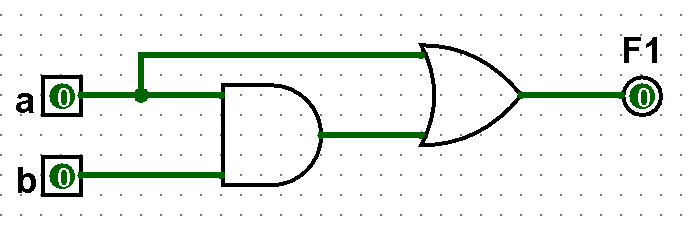
\includegraphics[width=0.8\textwidth]{F1.png}	
        \caption{Design of \textbf{$F_1$} in Logisim}
   \end{figure}
   
   \begin{figure}[H]
    \centering
        \includegraphics[width=\textwidth]{EasyEDA_part_1_F1.png}	
        \caption{Design of \textbf{$F_1$} in EasyEDA}
   \end{figure}
   
   \textbf{Design of $F_2$:} \\ 
    To design and implement $F_2$, we need to use two 2-input OR gates, a 2-input AND gate, a NOT gate.\\

    \begin{figure}[H]
    \centering
        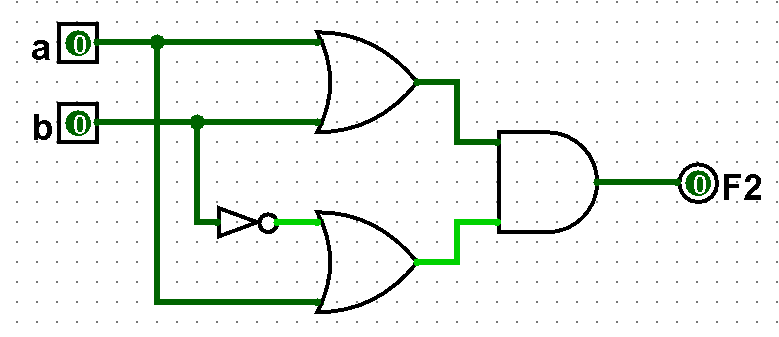
\includegraphics[width=0.8\textwidth]{F2.png}	
        \caption{Design of \textbf{$F_2$} in Logisim}
   \end{figure}
    
   \begin{figure}[H]
    \centering
        \includegraphics[width=\textwidth]{EasyEDA_part_1_F2.png}	
        \caption{Design of \textbf{$F_2$} in EasyEDA}
   \end{figure}
   
 
   To validate our designs of $F_1$ and $F_2$, we need to create truth tables of them. Both $F_1$ and $F_2$ functions have the same truth tables:\\
   \begin{figure}[H]
    \centering
        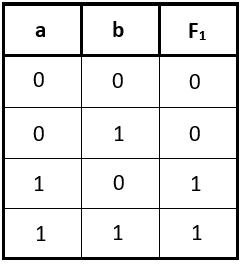
\includegraphics[width=0.25\textwidth]{f1truth.png}	
        \caption{Truth table of the function \textbf{$F_1$} and \textbf{$F_2$}}
   \end{figure}
   Our implementations of $F_1$ and $F_2$ are compatible with their truth table.\\
   Moreover, we can construct the same implementations with the help of \textbf{SPDT} switch which consists of three terminals, one is output and others are input terminals. Using switch button of \textbf{SPDT}, we are able to determine which input terminal will be connected to the output terminal.\\

   \textbf{Design of $F_1$ using SPDT switch:}\\
   \begin{figure}[H]
    \centering
        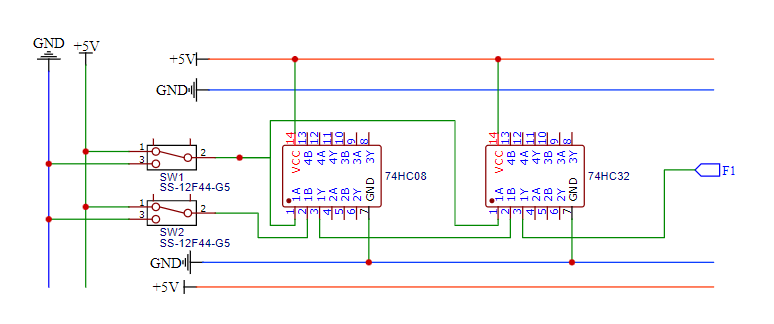
\includegraphics[width=0.9\textwidth]{F1ICspdt.png}	
        \caption{Design of $F_1$ using SPDT switch}
        \label{fig1}
   \end{figure}
   \textbf{Design of $F_2$ using SPDT switch:}\\
   \begin{figure}[H]
    \centering
        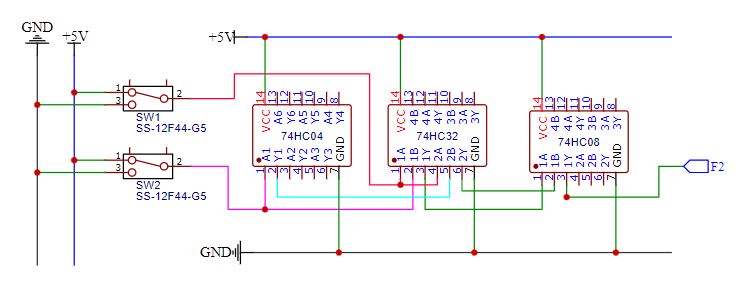
\includegraphics[width=0.9\textwidth]{F2ICspdt.png}	
        \caption{Design of $F_2$ using SPDT switch}
        
   \end{figure}
\end{itemize}
\begin{itemize}
    \item \textbf{Part 2:} A theorem is given as: $a + (a \cdot b) = a$. First, determine the dual of the given theorem and then, implement the functions for both sides of the dual theorem by using logic gates. Validate the truth of the theorem by comparing the changes in the outputs. \\
    
    First of all, the dual of a theorem is an expression created by replacing OR with AND, AND with OR, 1 with 0 and 0 with 1. Also, the order of operations should be preserved, so we need to put extra parentheses. In this formula, $(a \cdot b)$ is done first:
    
\begin{align*}
a + (a \cdot b) = a \tag{Original} \\
a \cdot (a+b) = a \tag{Dual} \\
\end{align*}

\begin{figure}[H]
\centering
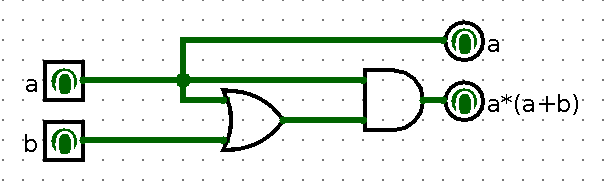
\includegraphics[width=0.8\textwidth]{Logisim_part_2.png}	
\caption{Design in Logisim}
\end{figure}

\begin{figure}[H]
\centering
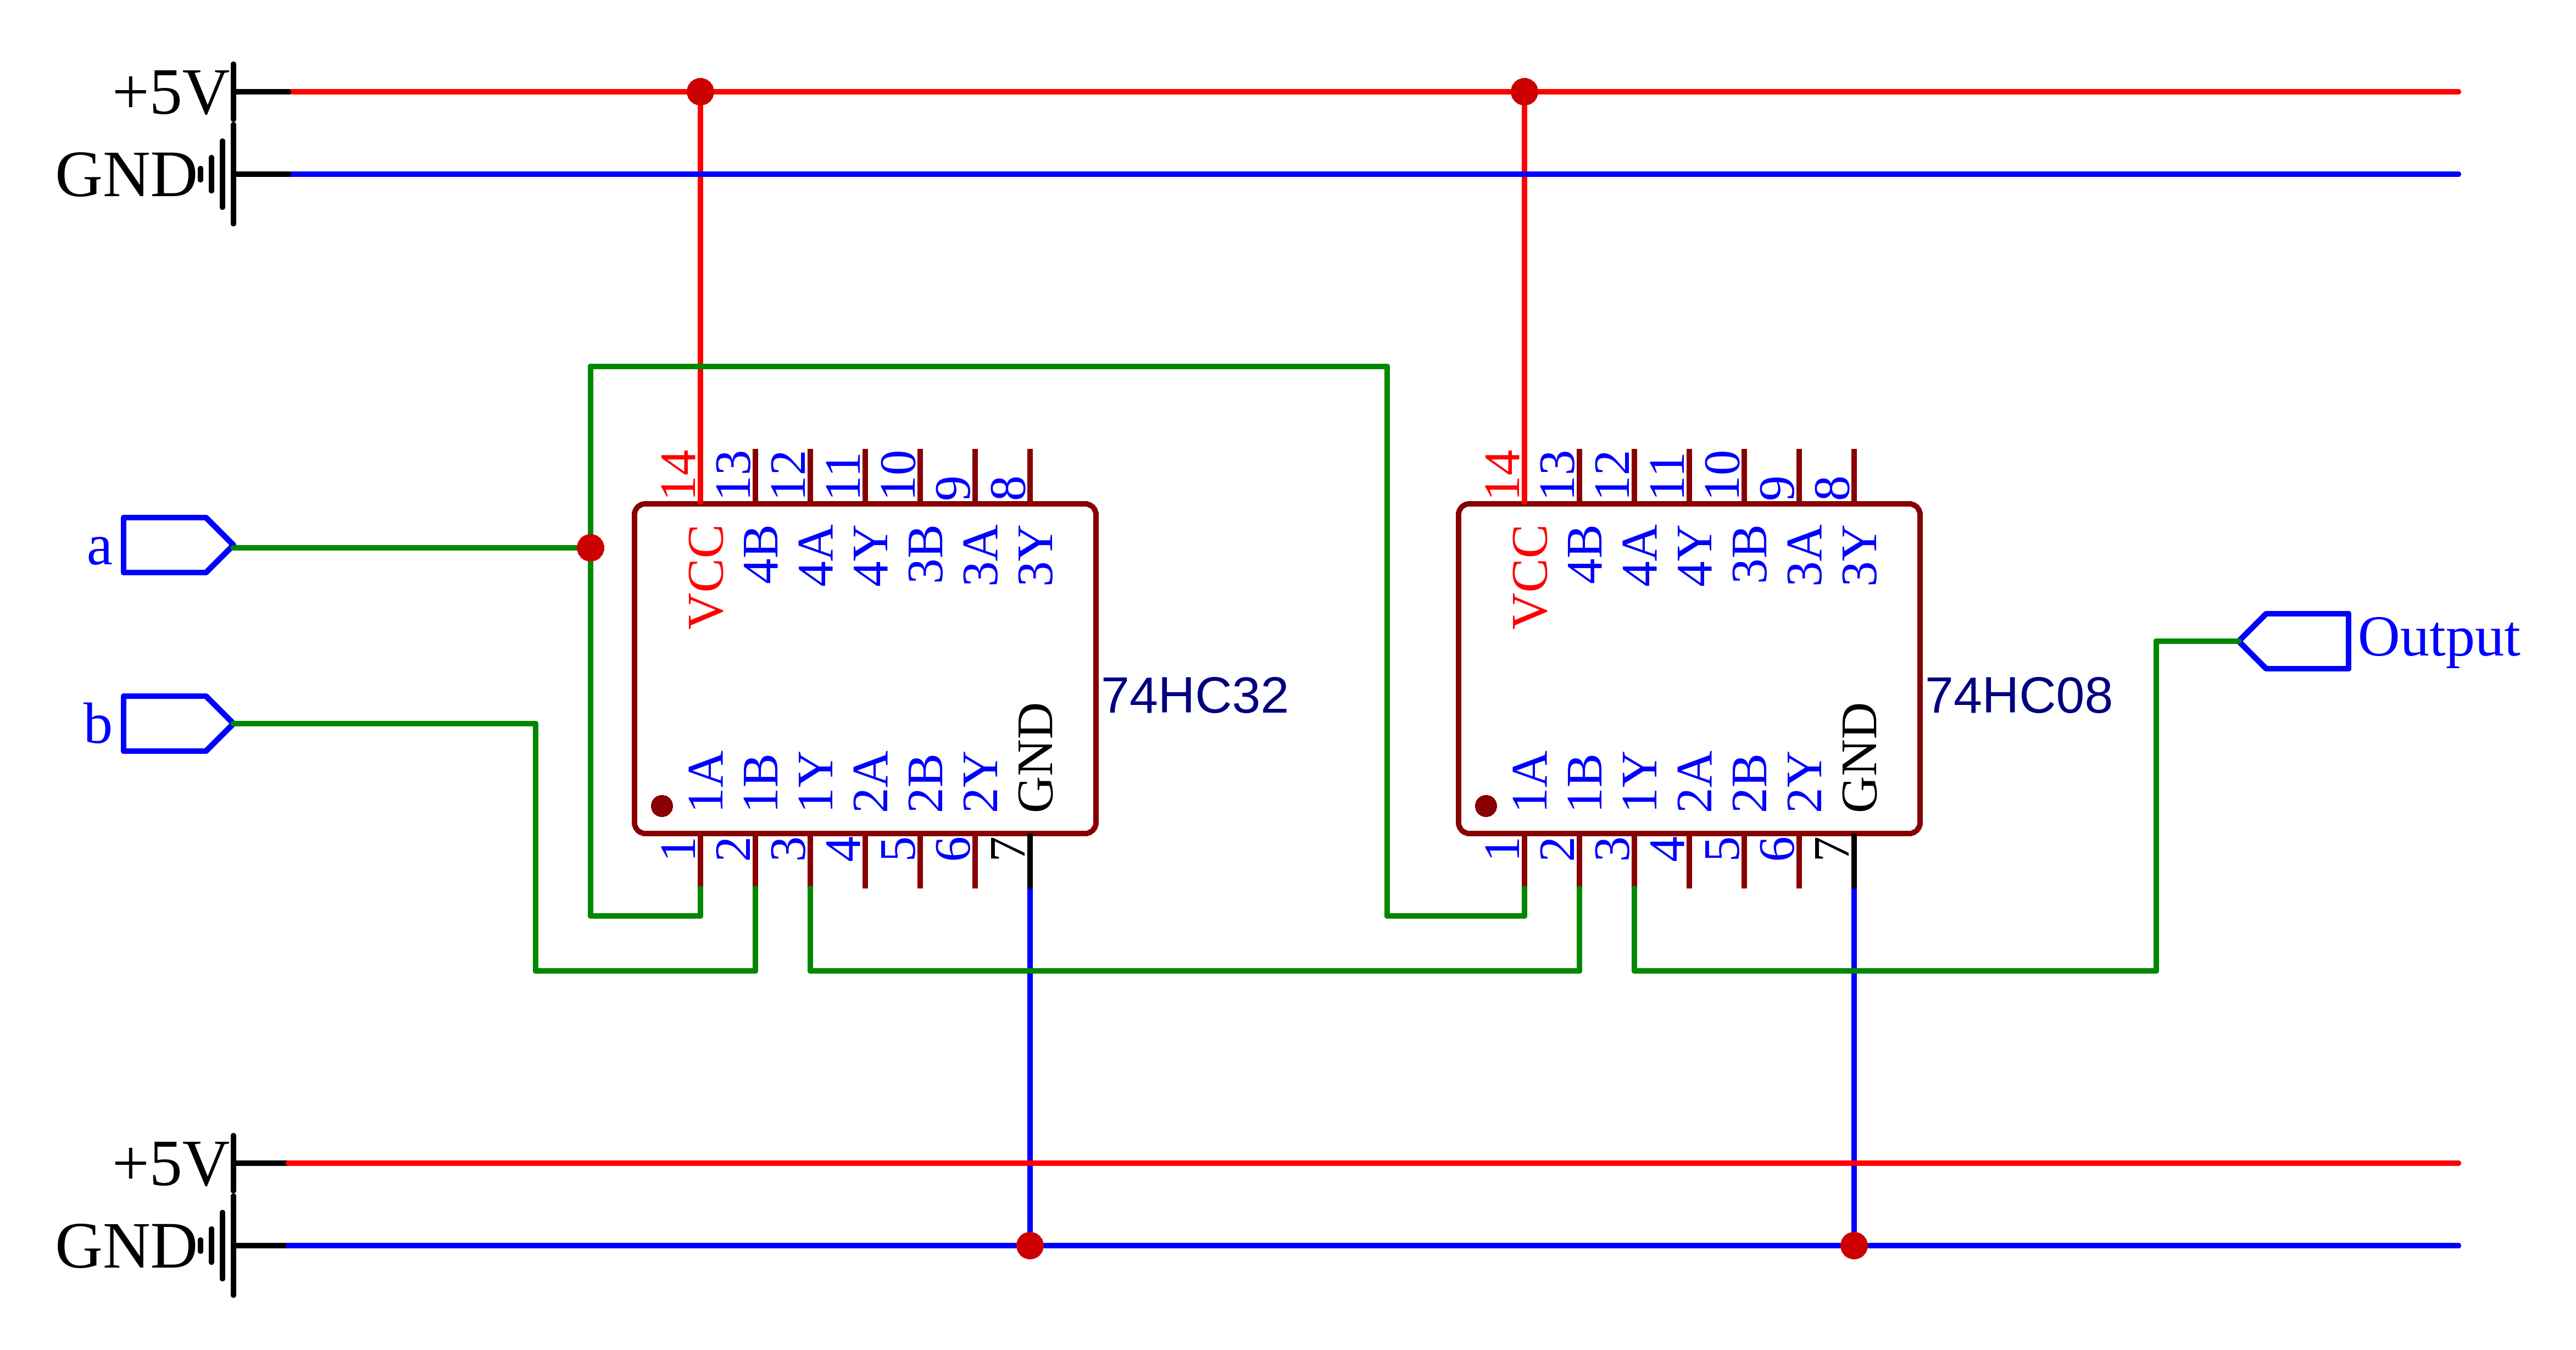
\includegraphics[width=\textwidth]{EasyEDA_part_2.png}	
\caption{Design in EasyEDA}
\end{figure}

To check validity of the dual theorem, the following truth table is constructed:

\begin{center}
\begin{tabular}{|c|c|c|c|c|c|}
\hline
$a$ & $b$ & $a \cdot b$ & $a+b$ & $a + a \cdot b$ & $a \cdot (a + b)$ \\
\hline
0 & 0 & 0 & 0 & 0 & 0 \\
0 & 1 & 0 & 1 & 0 & 0 \\
1 & 0 & 0 & 1 & 1 & 1 \\
1 & 1 & 1 & 1 & 1 & 1 \\
\hline
\end{tabular}
\end{center}
As it is clear from the table, the last two columns, which are the original expression's and its dual's left-hand side truth values, are identical to the first column, the right-hand side of the both equations. The equivalency of functions $a$ and $a \cdot (a+b)$ confirms the dual theorem. \\ 


\end{itemize}


\begin{itemize}
    \item \textbf{Part 3:} $F_3 (a, b, c) = ab + \overline{a}c$ is given. First, determine the complement of the given function ($F_3$). Then, implement the circuit which realizes the complementary function ($\overline{F_3}$). Validate your implementation by using the truth table.\\

    In the first step, we find the complement of the given function $F_3$ by applying \textbf{De Morgan's} rule.\\
    
    $\overline{F_3 (a, b, c)} = \overline{ab + \overline{a}c}$ \\
    
    $\overline{F_3 (a, b, c)} = (\overline{a} + \overline{b}) . (a + \overline{c})$\\
    
    In the second step, we implement the circuit which realizes the function $\overline{F_3}$ using logic gates and ICs.\\

    \begin{figure}[H]
    \centering
        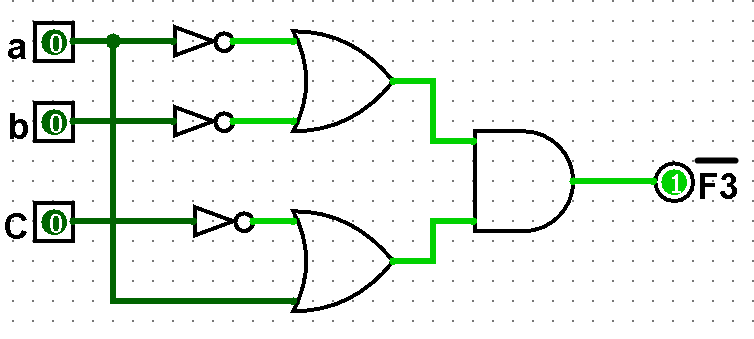
\includegraphics[width=0.8\textwidth]{F3comp.png}	
        \caption{Design of \textbf{$\overline{F_3}$} in Logisim}
   \end{figure}
   	
	\begin{figure}[H]
    \centering
        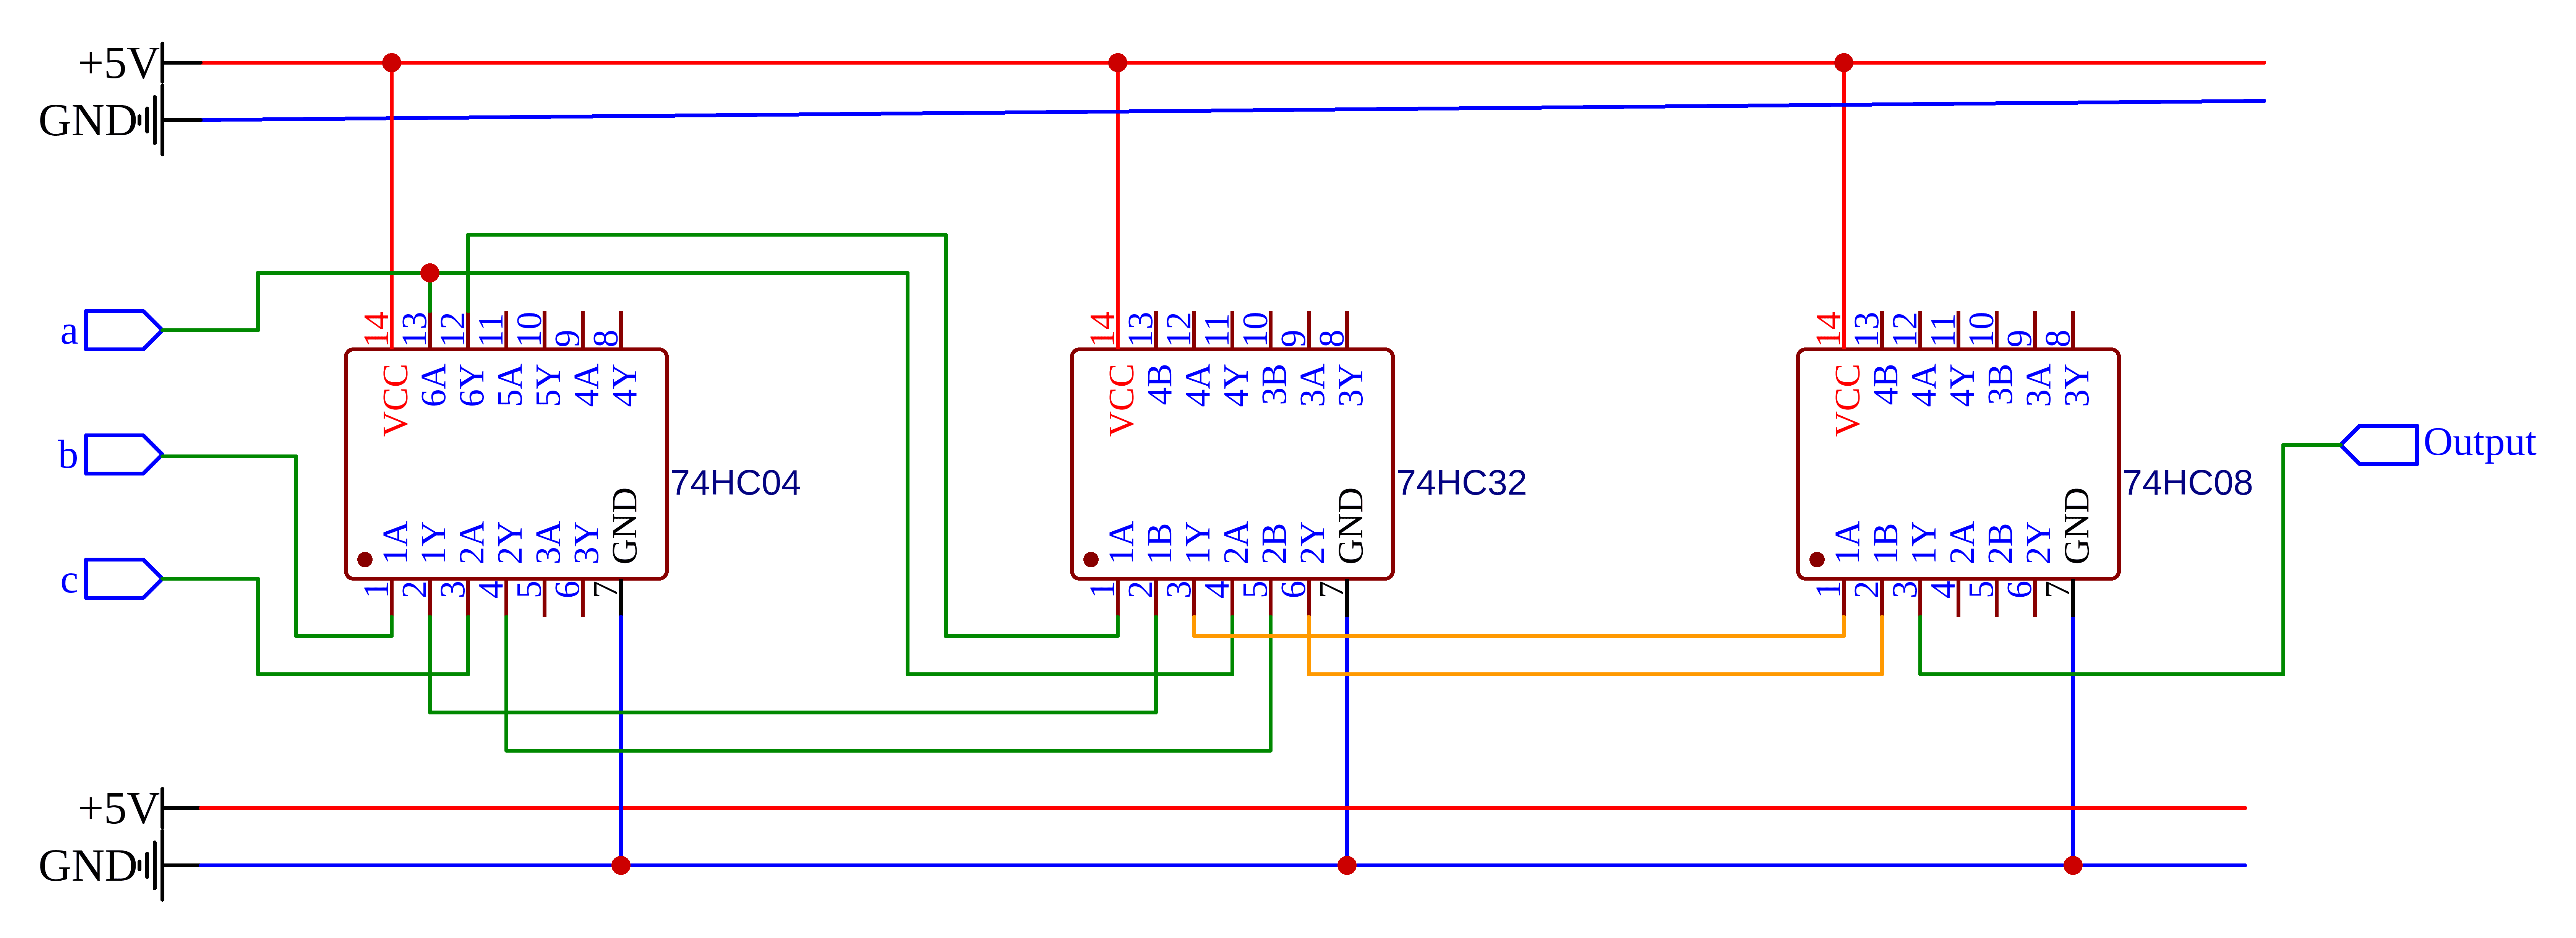
\includegraphics[width=\textwidth]{EasyEDA_part_3.png}	
        \caption{Design of \textbf{$\overline{F_3}$} in EasyEDA}        
	\end{figure}   
   
   In the third step, we validate our implementation of the function $\overline{F_3}$ using truth table.\\
    \begin{figure}[H]
    \centering
        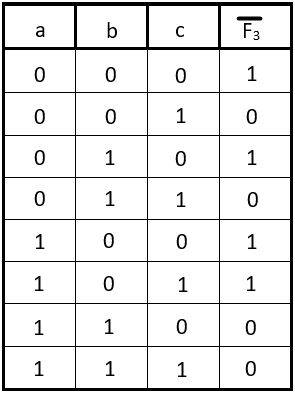
\includegraphics[width=0.3\textwidth]{truth.png}	
        \caption{Truth table of \textbf{$\overline{F_3}$}}
        
   \end{figure}
    According to the truth table, our implementation is correct.
\end{itemize}

\begin{itemize}
    \item \textbf{Part 4:} A basic logical function $F_4$ is defined as follows.	
    $ F_4(a, b, c, d) = \cup_1 (1, 2, 5, 6, 9, 10, 13, 14) $.
    First, simplify given logical function and implement the simplified expression using logic gates. Validate your circuit by observing the outputs for each possible input. \\

Simplification is done using Karnaugh map. The result suggests only two prime implicants as show below:  

\begin{center}
  \begin{tabular}{c}
   \begin{tabular}{|c|c|}
  \hline
    ABCD & $F_4$ \\
    \hline
    0000 & 0 \\
    0001 & 1 \\
    0010 & 1 \\
    0011 & 0 \\
    0100 & 0 \\
    0101 & 1 \\
    0110 & 1 \\
    0111 & 0 \\
    1000 & 0 \\
    1001 & 1 \\
    1010 & 1 \\
    1011 & 0 \\
    1100 & 0 \\
    1101 & 1 \\
    1110 & 1 \\
    1111 & 0 \\
    \hline
  \end{tabular}
    
    $\quad$
    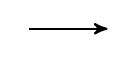
\begin{tikzpicture}[->,>=stealth', thick]
      \draw[->] (0,0) -- (1,0);
    \end{tikzpicture}
    $\quad$
    \begin{NiceTabular}{|w{l}{1cm}|c|c|c|c|}\hline
%\rule[-5mm]{5mm}{0cm}
\diagbox{AB}{CD}&
\Block{}{00}&\Block{}{01}&\Block{}{11}&\Block{}{10}\\
\hline
00 & 0 & 1 & 0 & 1\\
\hline
01 & 0 & 1 & 0 & 1\\
\hline
11 & 0 & 1 & 0 & 1\\
\hline
10 & 0 & 1 & 0 & 1\\
\hline
\end{NiceTabular}
    $\quad$
    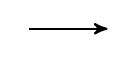
\begin{tikzpicture}[->,>=stealth', thick]
      \draw[->] (0,0) -- (1,0);
    \end{tikzpicture}
    $\quad$
    
     $ C\overline{D} + \overline{C}D $
  \end{tabular}
\end{center}

With the formula obtained, the following circuits are designed:

\begin{figure}[H]
    \centering
        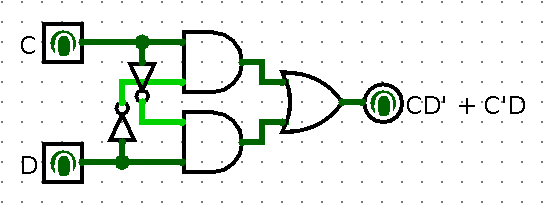
\includegraphics[width=0.8\textwidth]{Logisim_part_4.png}	
        \caption{Design of \textbf{$F_4$} in Logisim}
   \end{figure}
   
	\begin{figure}[H]
    \centering
        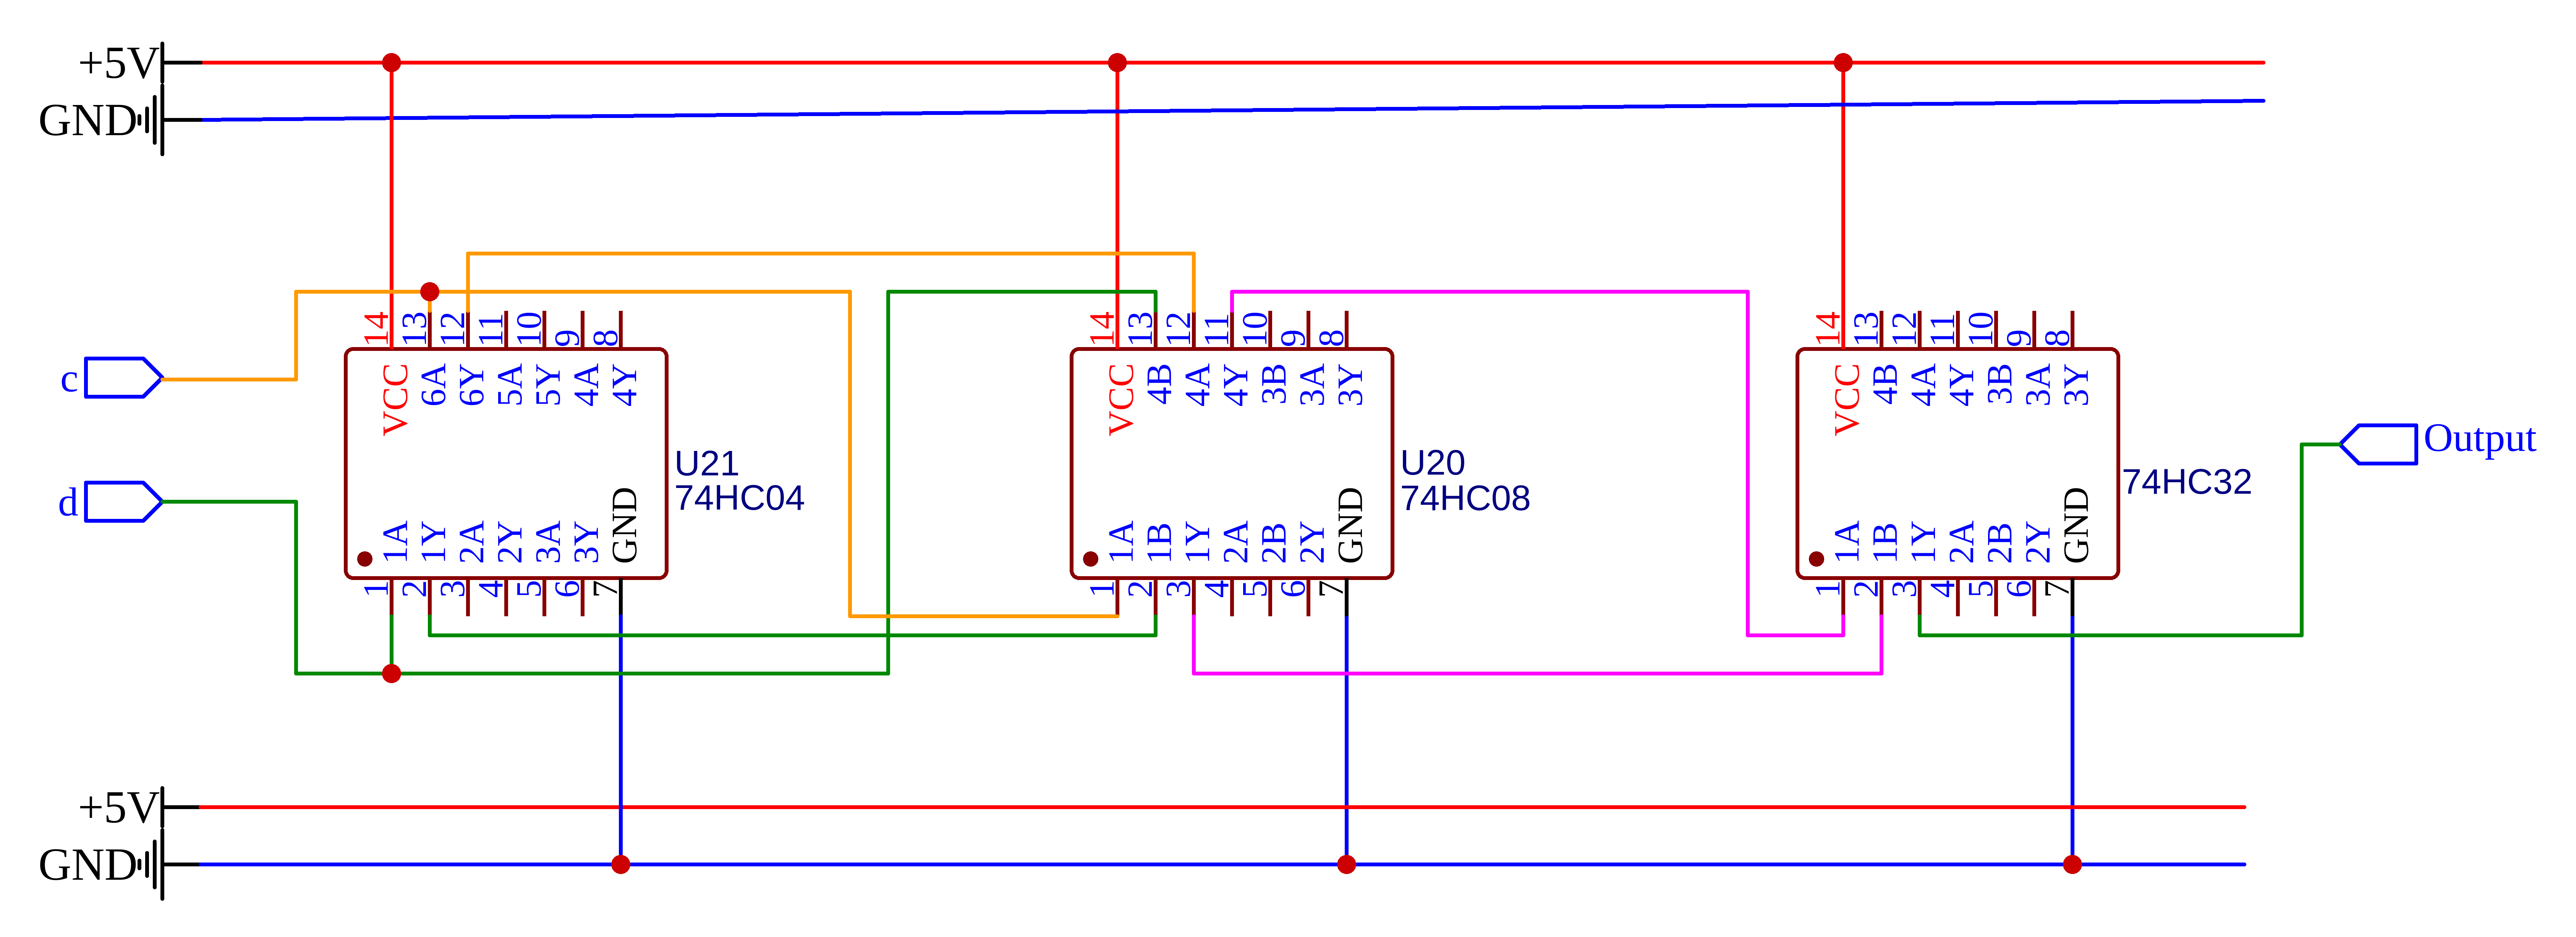
\includegraphics[width=\textwidth]{EasyEDA_part_4.png}	
        \caption{Design of \textbf{$F_4$} in EasyEDA}        
	\end{figure}  

\end{itemize}
\begin{itemize}
    \item \textbf{Part 5:}
    \begin{itemize}
        \item \textbf{By using voltmeter, observe $V_{cc}$ and $G_{nd}$ voltages:}\\
    Using voltmeter, we can observe the voltage difference between $V_{cc}$ and $G_{nd}$. Also, we can alter the voltage difference to a specific value with the help of CADET interface. In our experiments, we set $V_{cc}$ to 5V and $G_{nd}$ to 0V, since these values are optimal for the ICs we use in our implementations. Also, we observed $V_{cc}$ and $G_{nd}$ voltages using voltmeter.
    \end{itemize}
    \begin{itemize}
        \item \textbf{By using potentiometer, build a resistance in 8 Kohm:}\\
    In CADET, we are able to specify a resistance value benefeting from potentiometer. To achieve this, we also need an ohmmeter to observe current resistance. So, in our experiment, we built a resistance value of 8 Kohm by adjusting the wiper of potentiometer in CADET. Also, we observed the value of the resistance simultaneously through the ohmmeter.
    \end{itemize}
    \begin{itemize}
        \item \textbf{Show ”27” in two seven segment display by giving an input using 8 switches:}\\
    In this part of our experiment, we used eight different switches in CADET, four switches were used to display "2" and others were used to display "7" in seven segment display. During the experiment, we explored that our switches were operating as binary number digits and display the binary value as its corresponding decimal integer; before explaining in detail, we should examine our switch components:\\
    \begin{figure}[H]
    \centering
        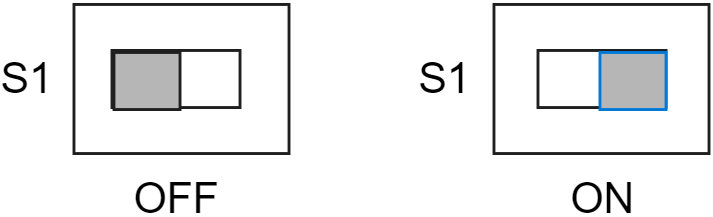
\includegraphics[width=0.6\textwidth]{switch.png}	
        \caption{Switch component}
        
   \end{figure}
   
   Each switch corresponds to one single digit in our binary number. For instance, S0 (switch 0) determines the value of first digit in our binary number. If S0 is OFF, then first digit of the binary number is also 0. To illustrate the working principle of switches in a better way, we can use the schema below:
   \begin{figure}[H]
    \centering
        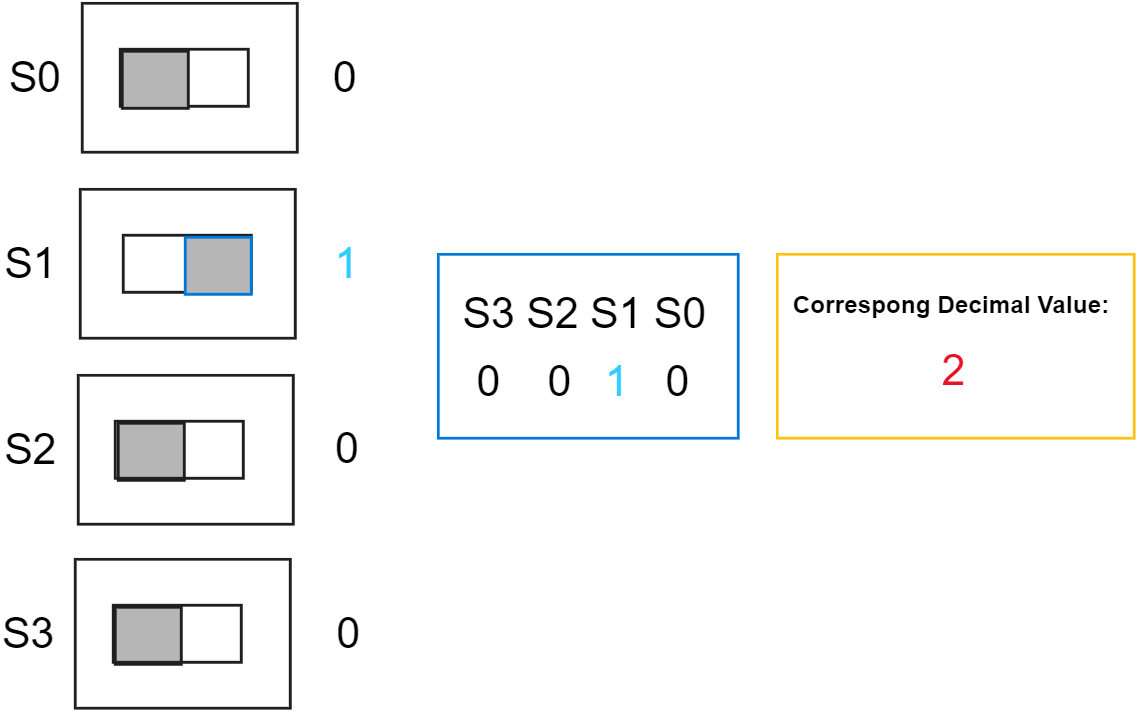
\includegraphics[width=0.8\textwidth]{display2.png}	
        \caption{How to display "2" using switches}
        
   \end{figure}
   Therefore, in order to display "2", we set S1 to 1 (ON) and others are set to 0 (OFF).\\

   Similarly, to display "7", we set S0, S1, S2 to 1 (ON), and S3 to 0 (OFF):
   \begin{figure}[H]
    \centering
        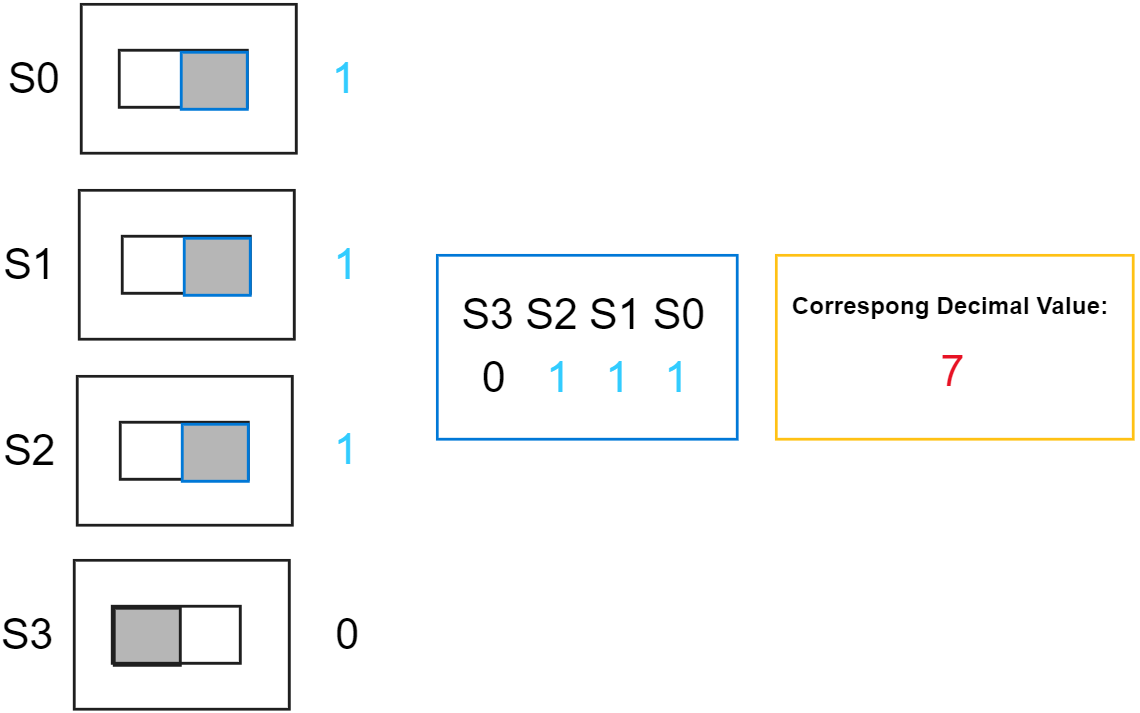
\includegraphics[width=0.8\textwidth]{display7.png}	
        \caption{How to display "7" using switches}
        
   \end{figure}

   \textbf{Implementation of seven segment display using ICs:}
   \begin{figure}[H]
    \centering
        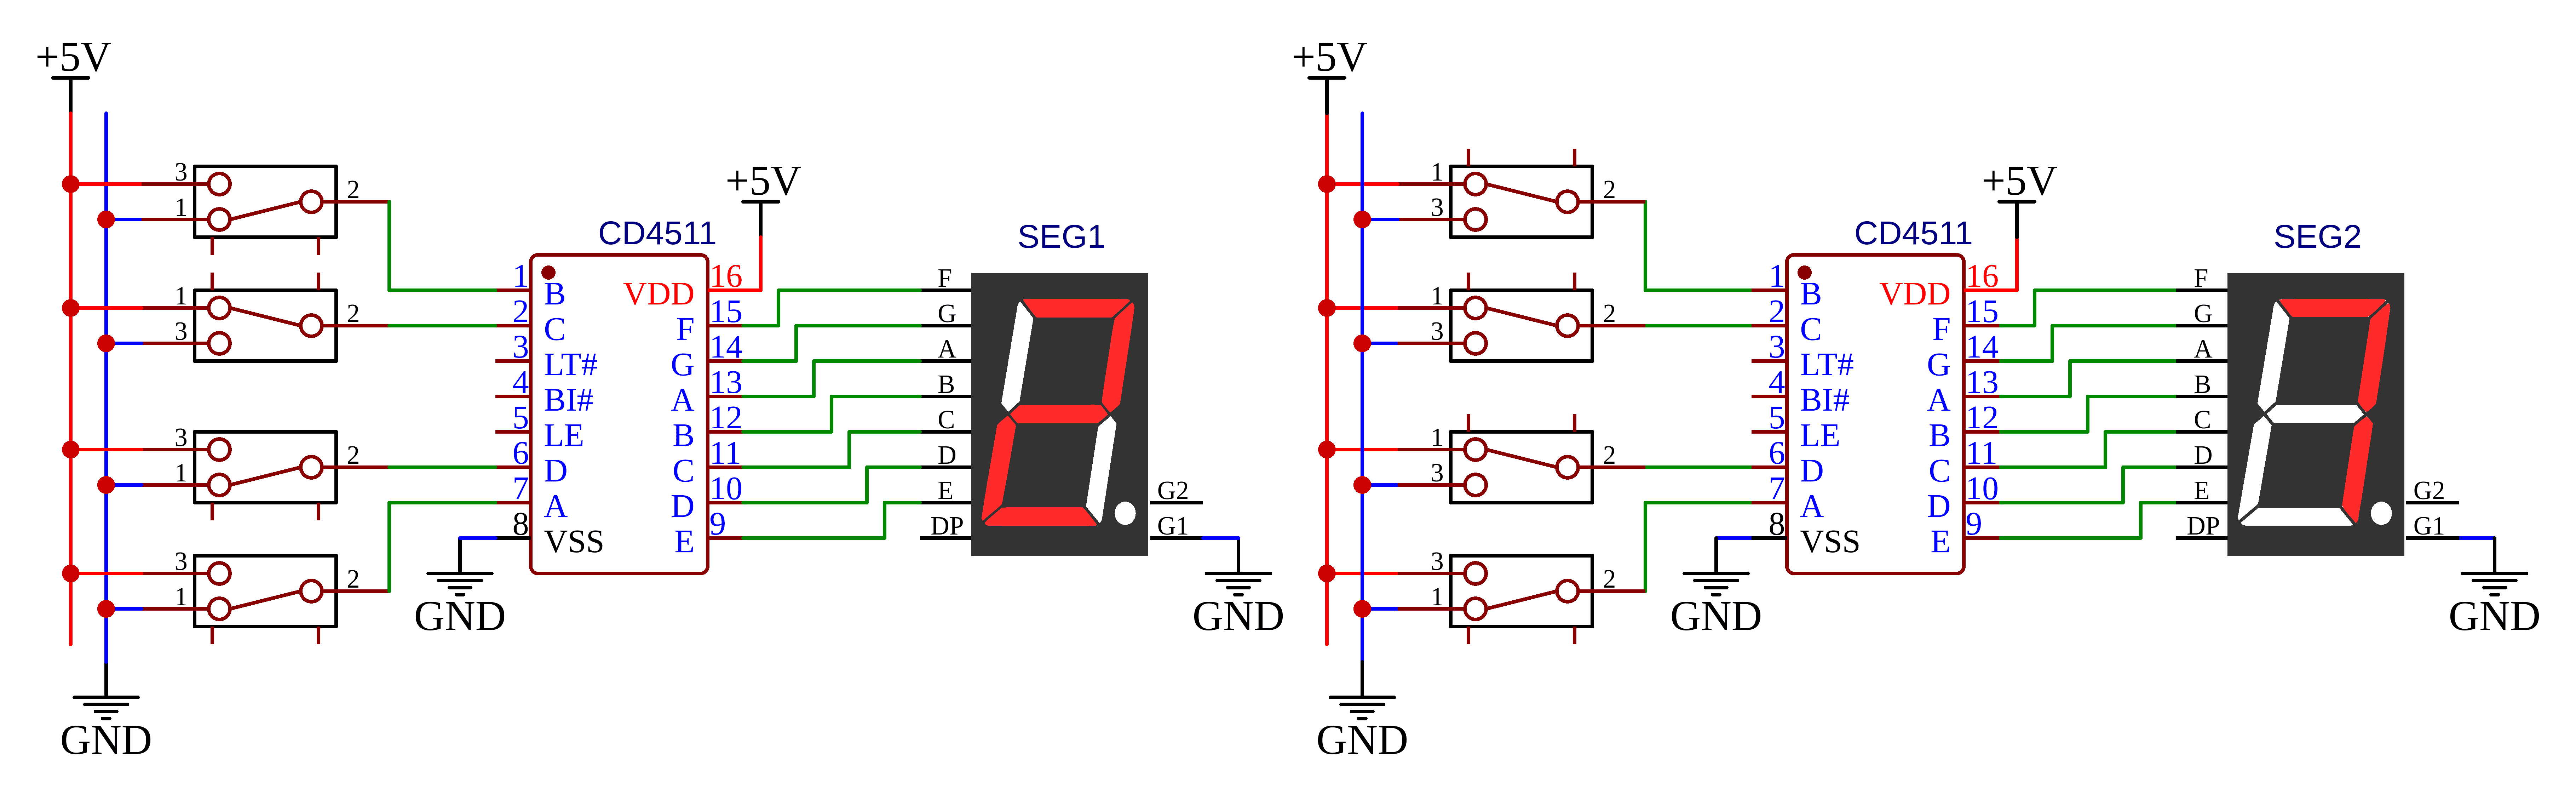
\includegraphics[width=0.9\textwidth]{part5.png}	
        \caption{How to display "27" in two segment display using 8 switches}
        
   \end{figure}
    \end{itemize}
    
\end{itemize}

\begin{itemize}
    \item \textbf{Part 6:}
    C.A.D.E.T. has a built-in 200kHz function generator with a number of knobs, which adjust the function to any desired characteristics. By changing the parameters, functions of different shapes were obtained:
    
\begin{figure}[H]
\begin{subfigure}{0.5\textwidth}
\centering
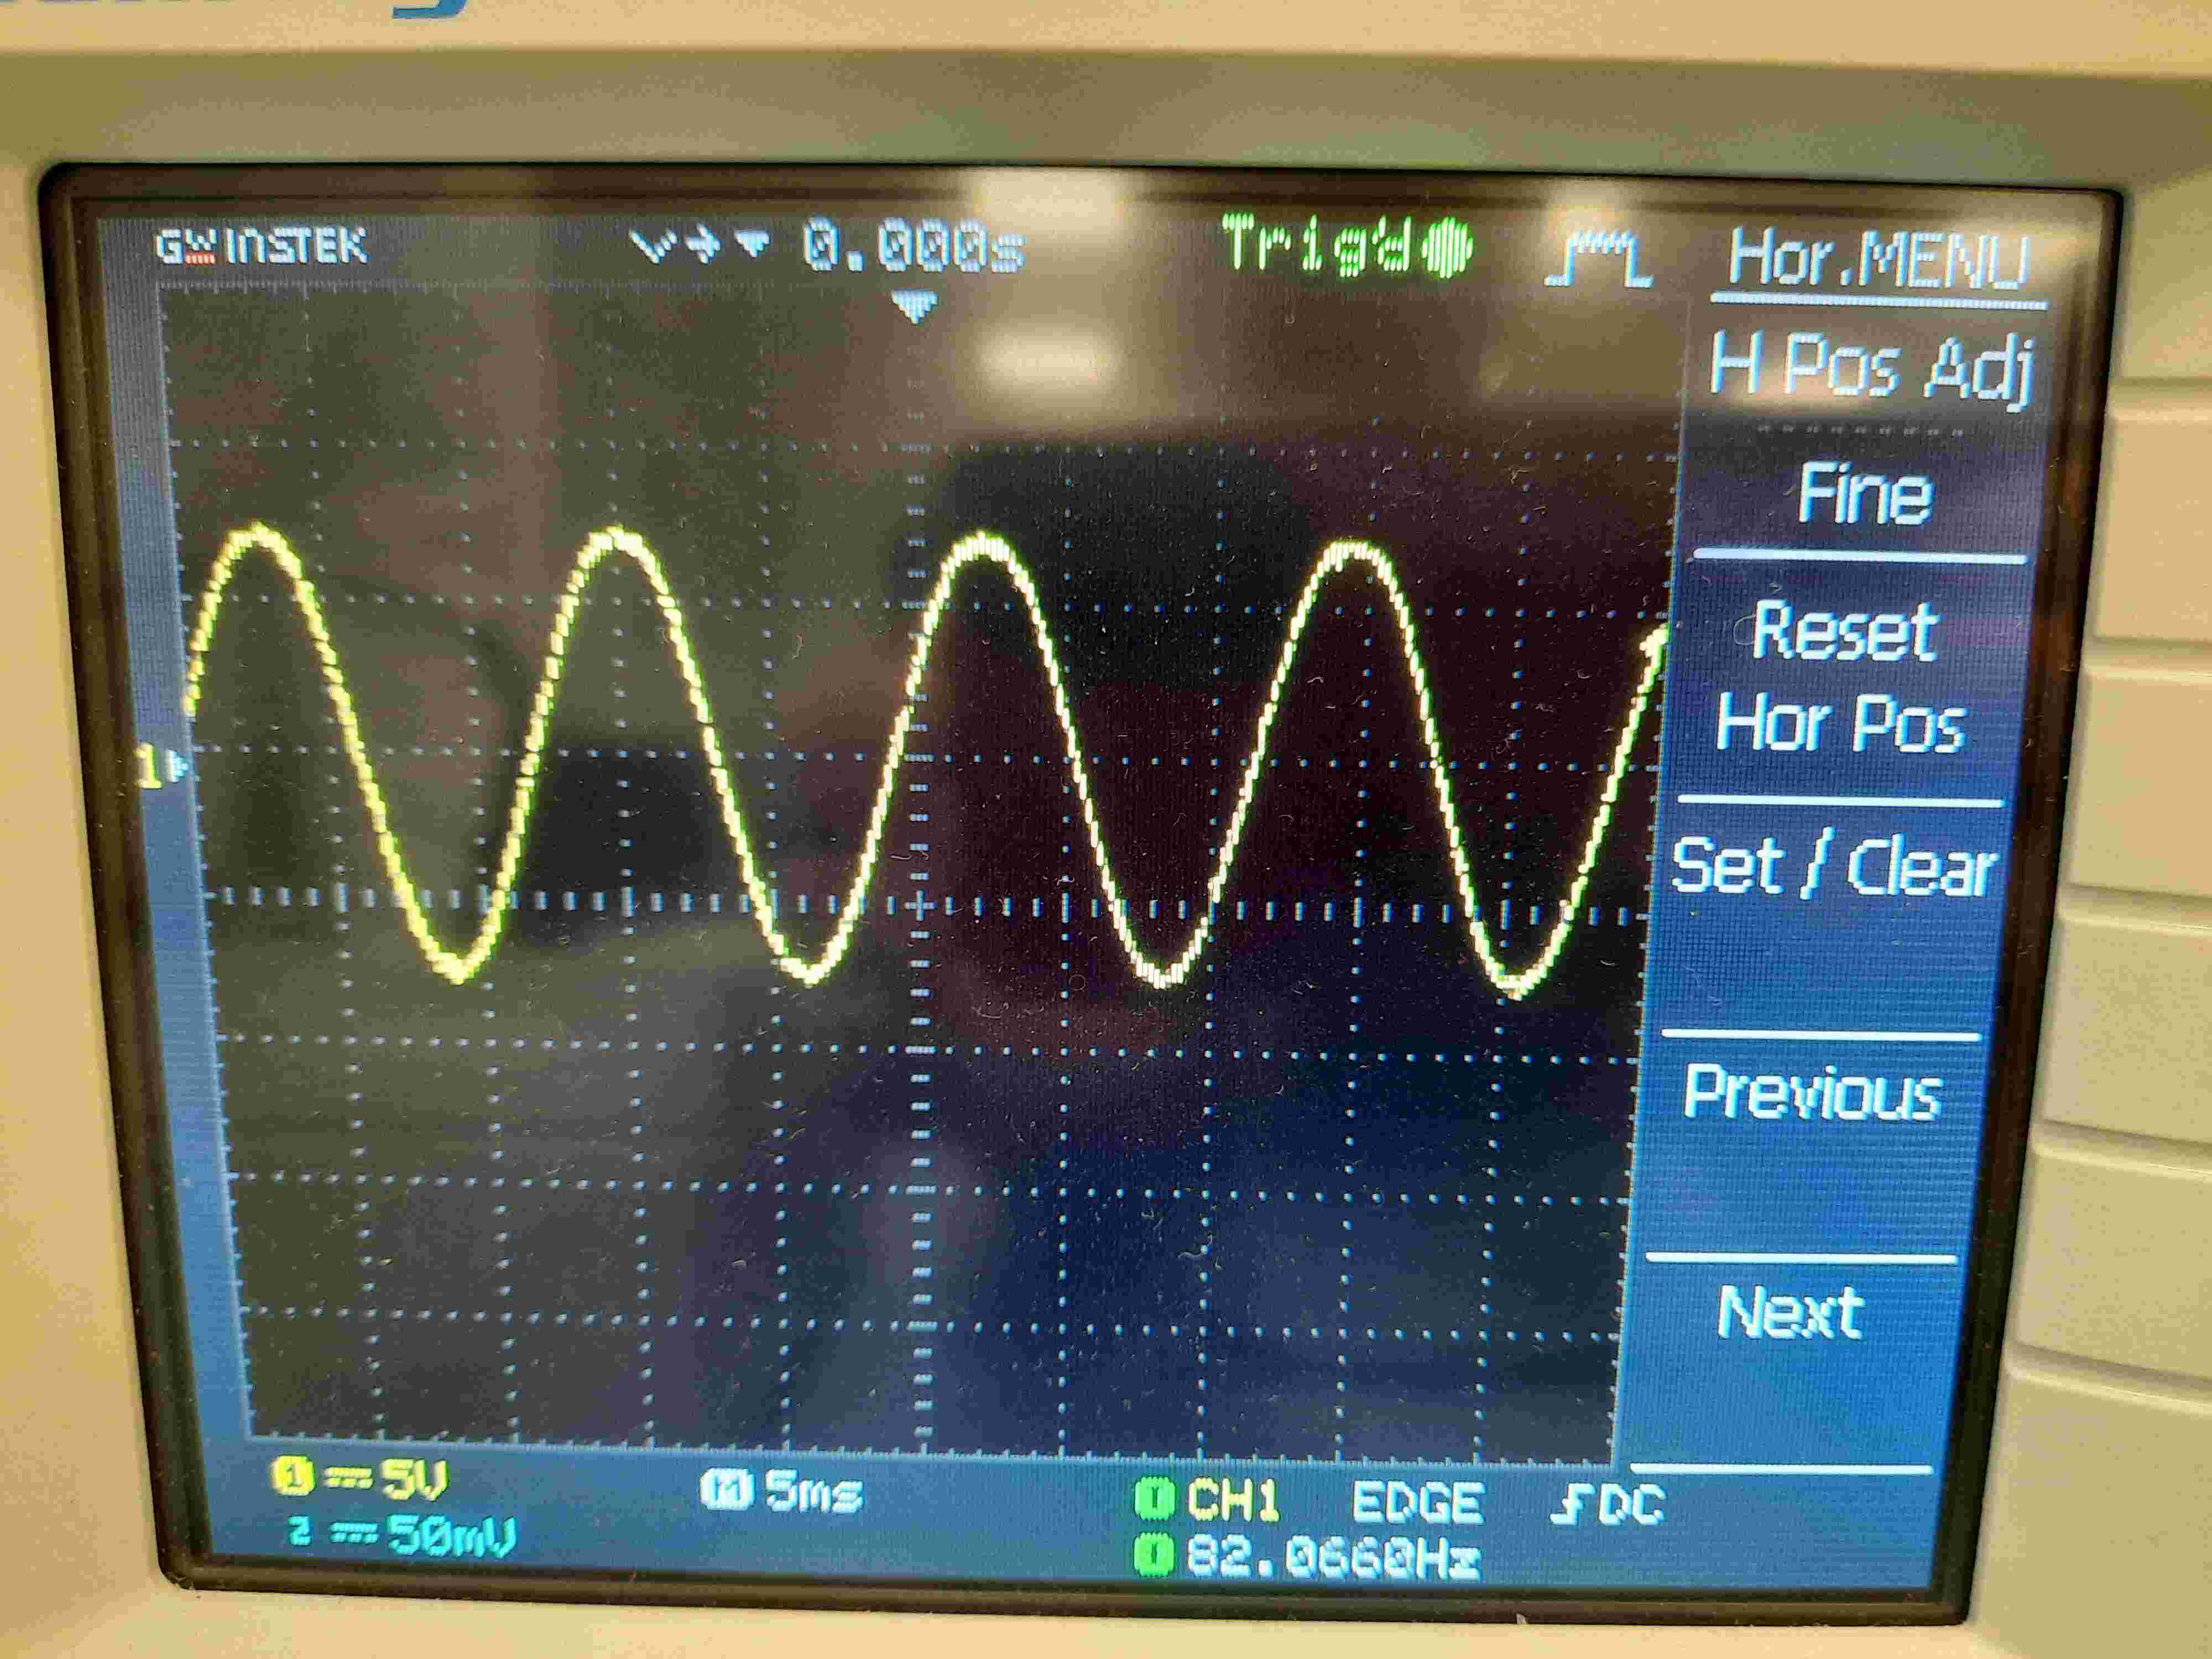
\includegraphics[width=.95\linewidth]{sine_wave_1.jpg}
\end{subfigure}%
\begin{subfigure}{0.5\textwidth}
\centering
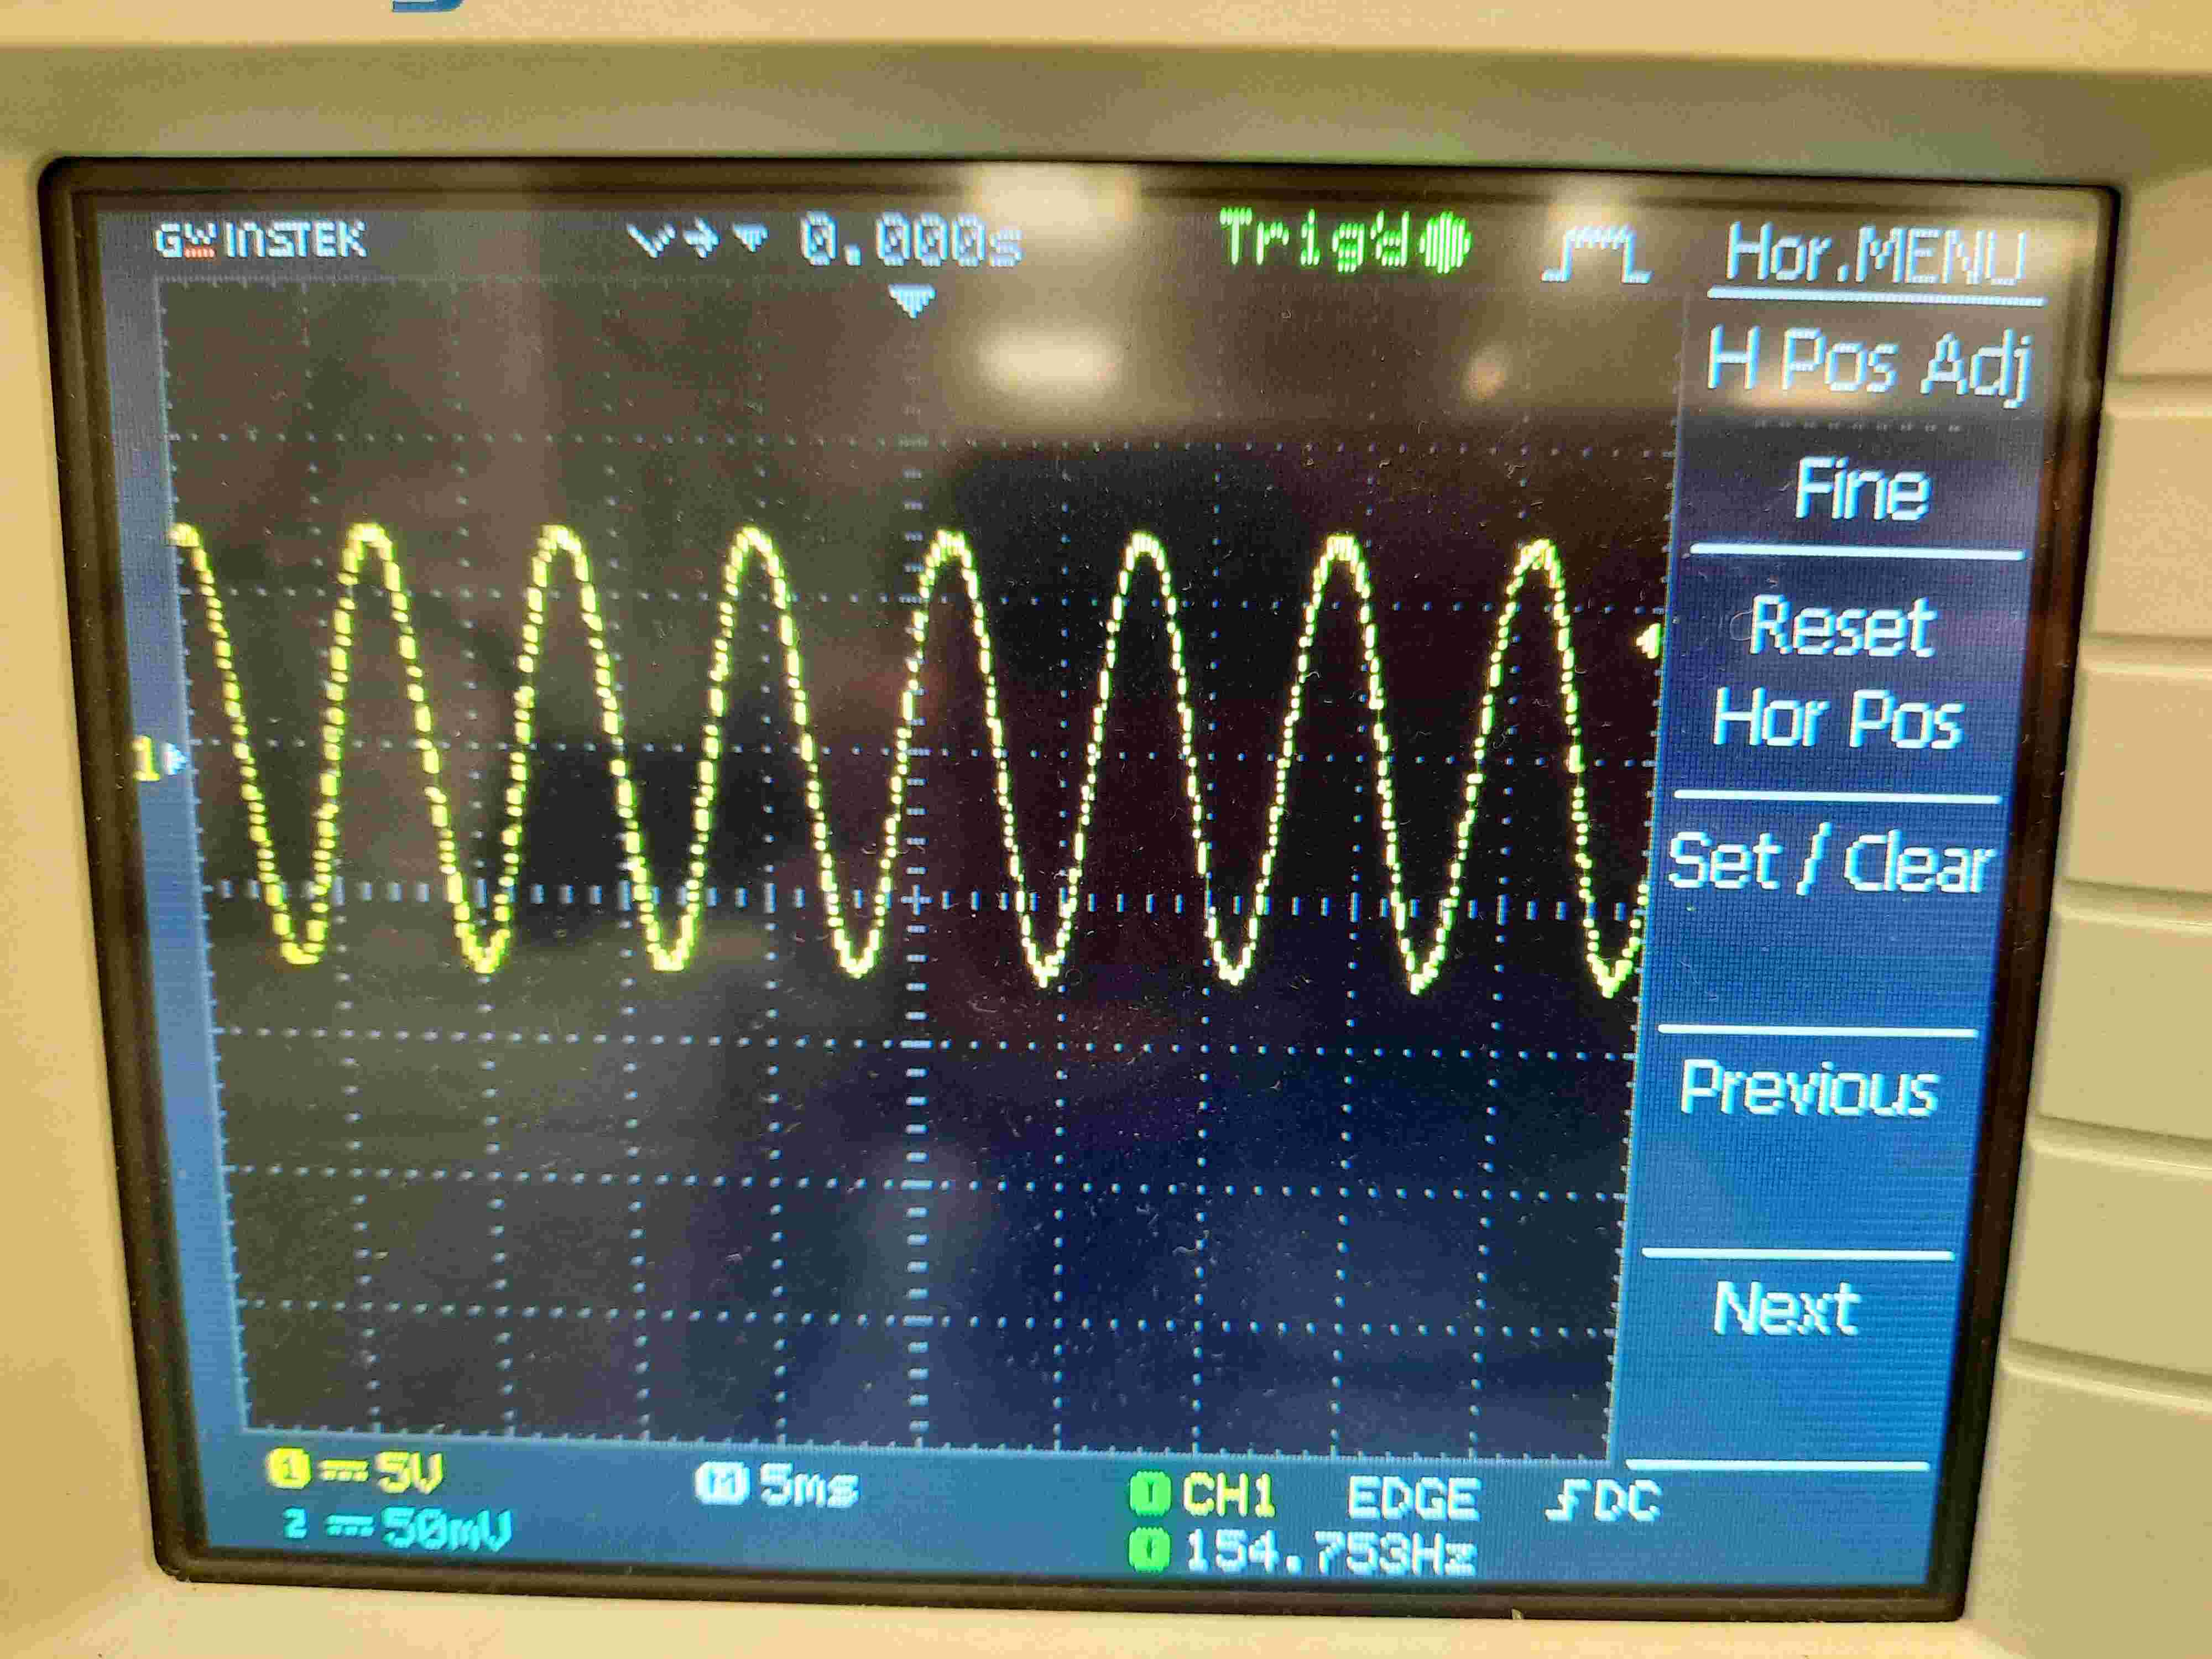
\includegraphics[width=.95\linewidth]{sine_wave_2.jpg}
\end{subfigure}
\caption{Sine waves generated}
\end{figure}

\begin{figure}[H]
\begin{subfigure}{0.5\textwidth}
\centering
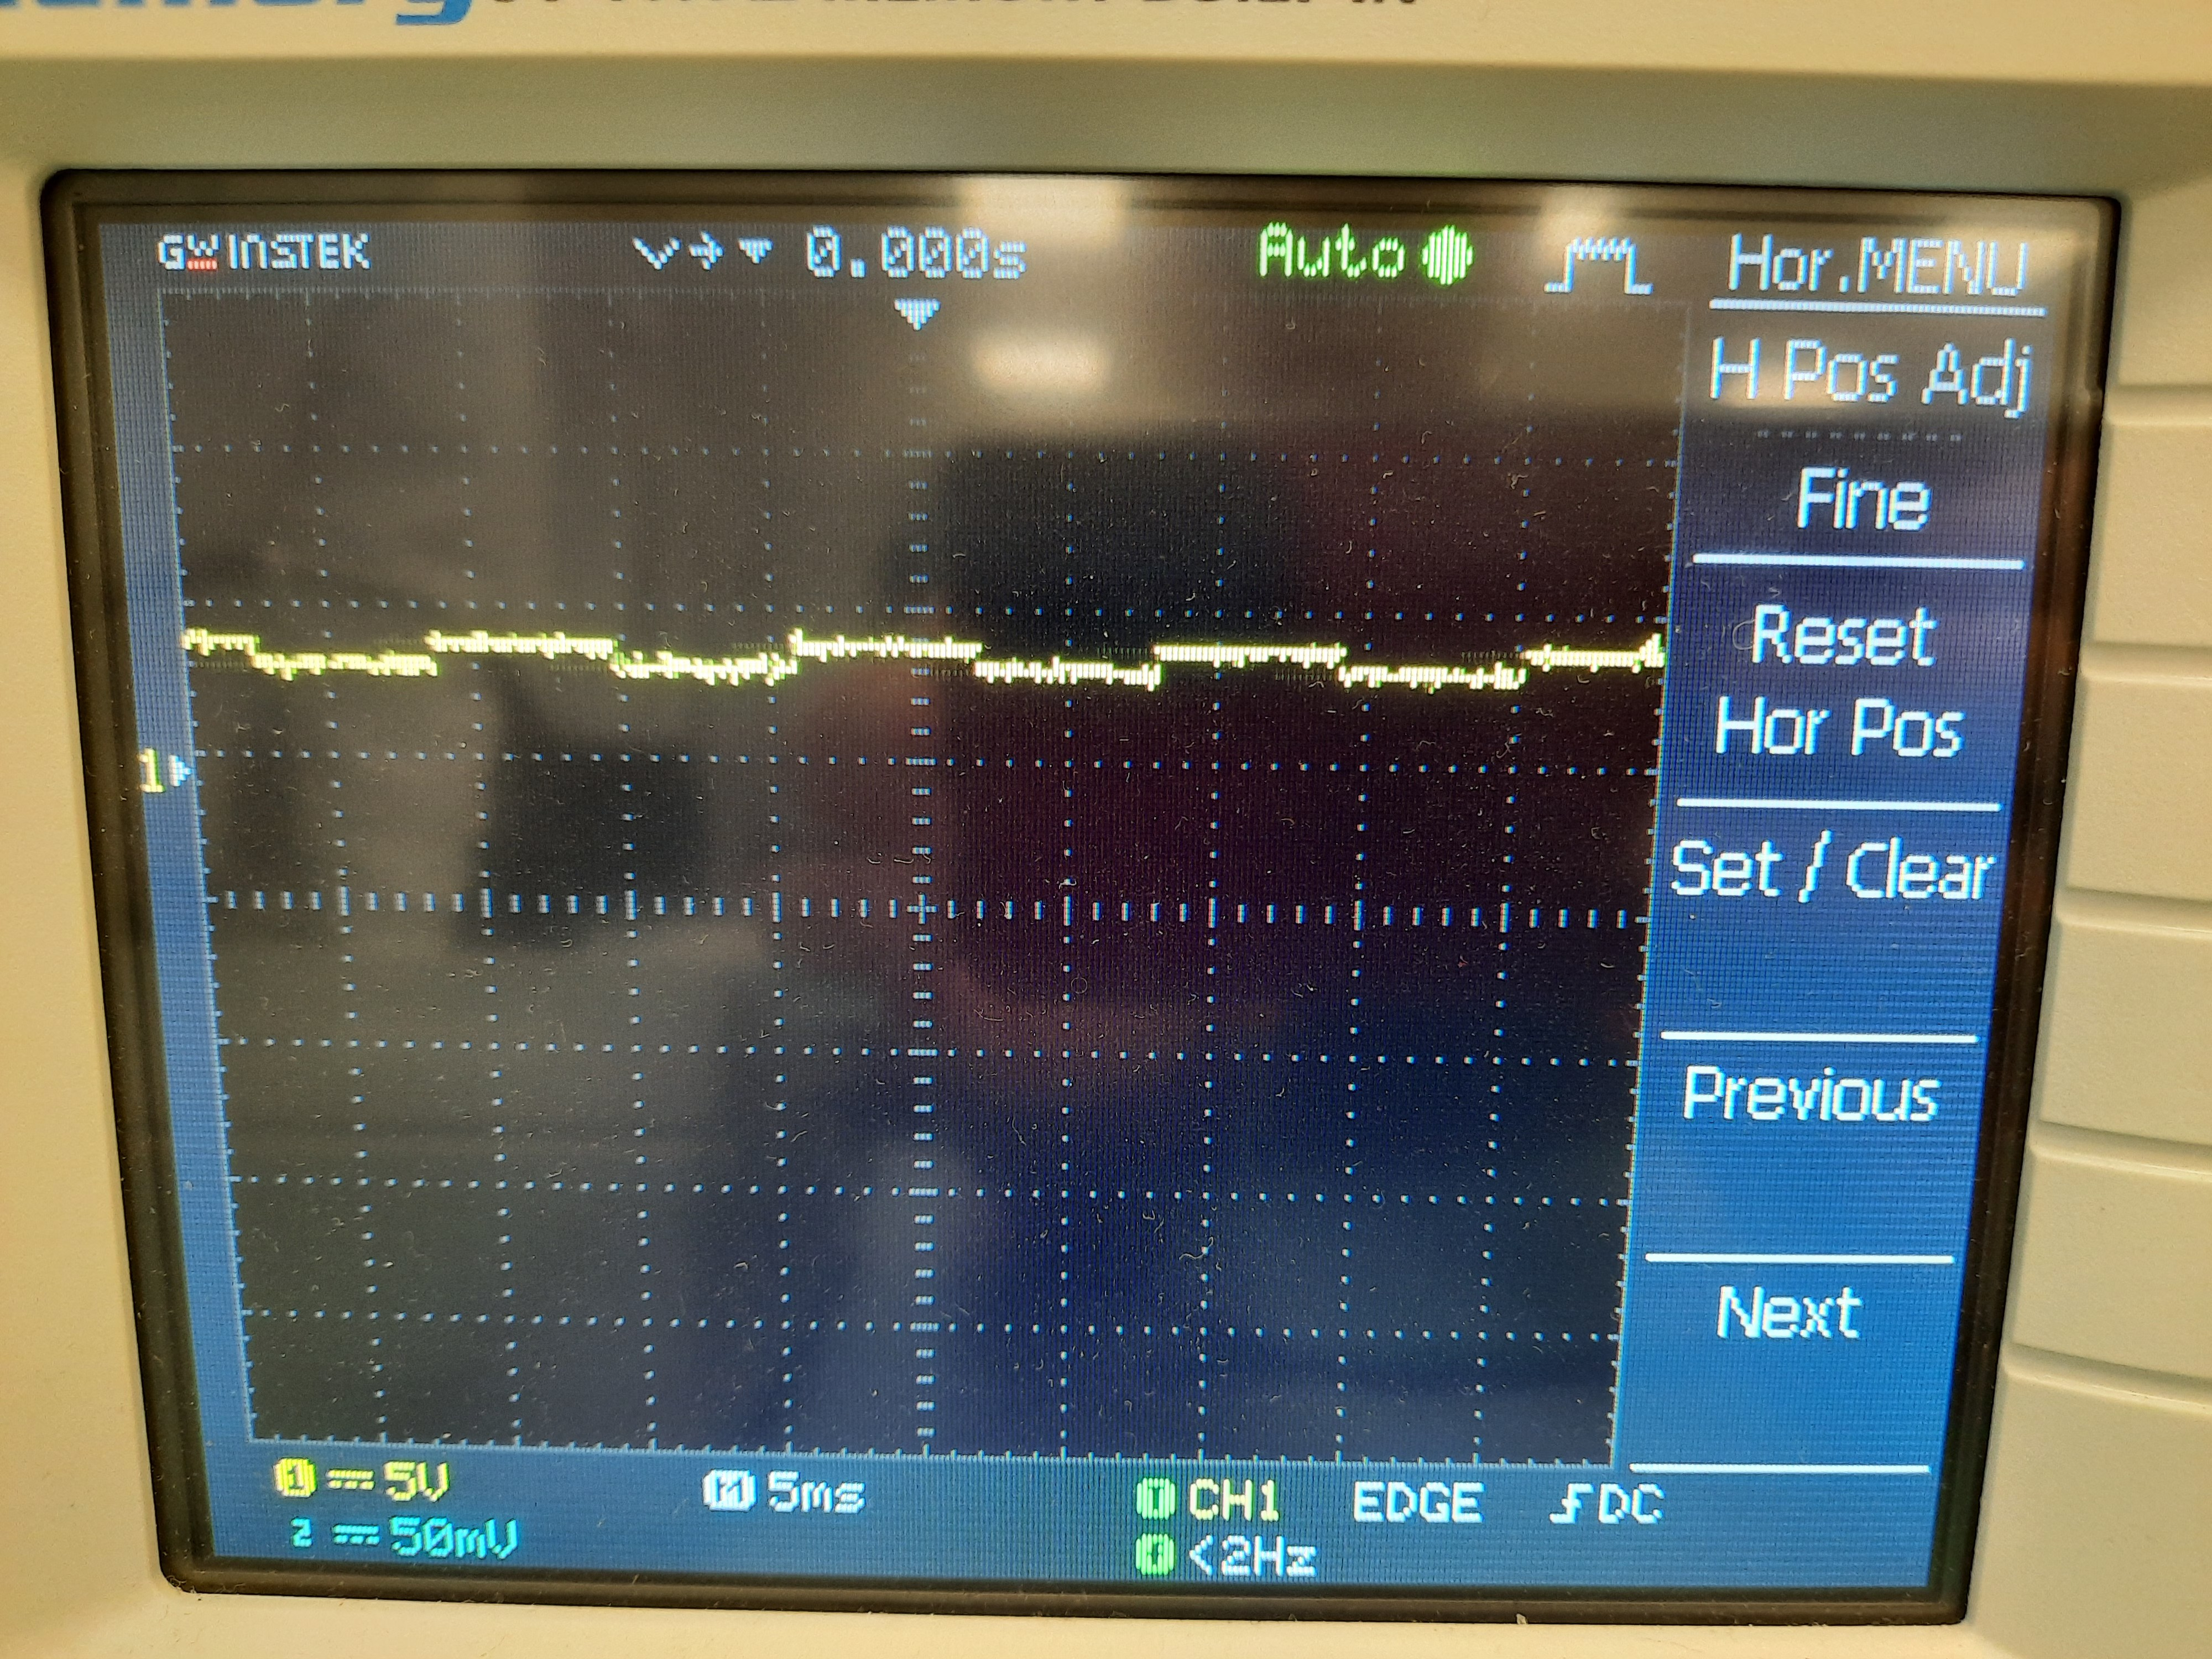
\includegraphics[width=.95\linewidth]{square_wave_1.jpg}
\end{subfigure}%
\begin{subfigure}{0.5\textwidth}
\centering
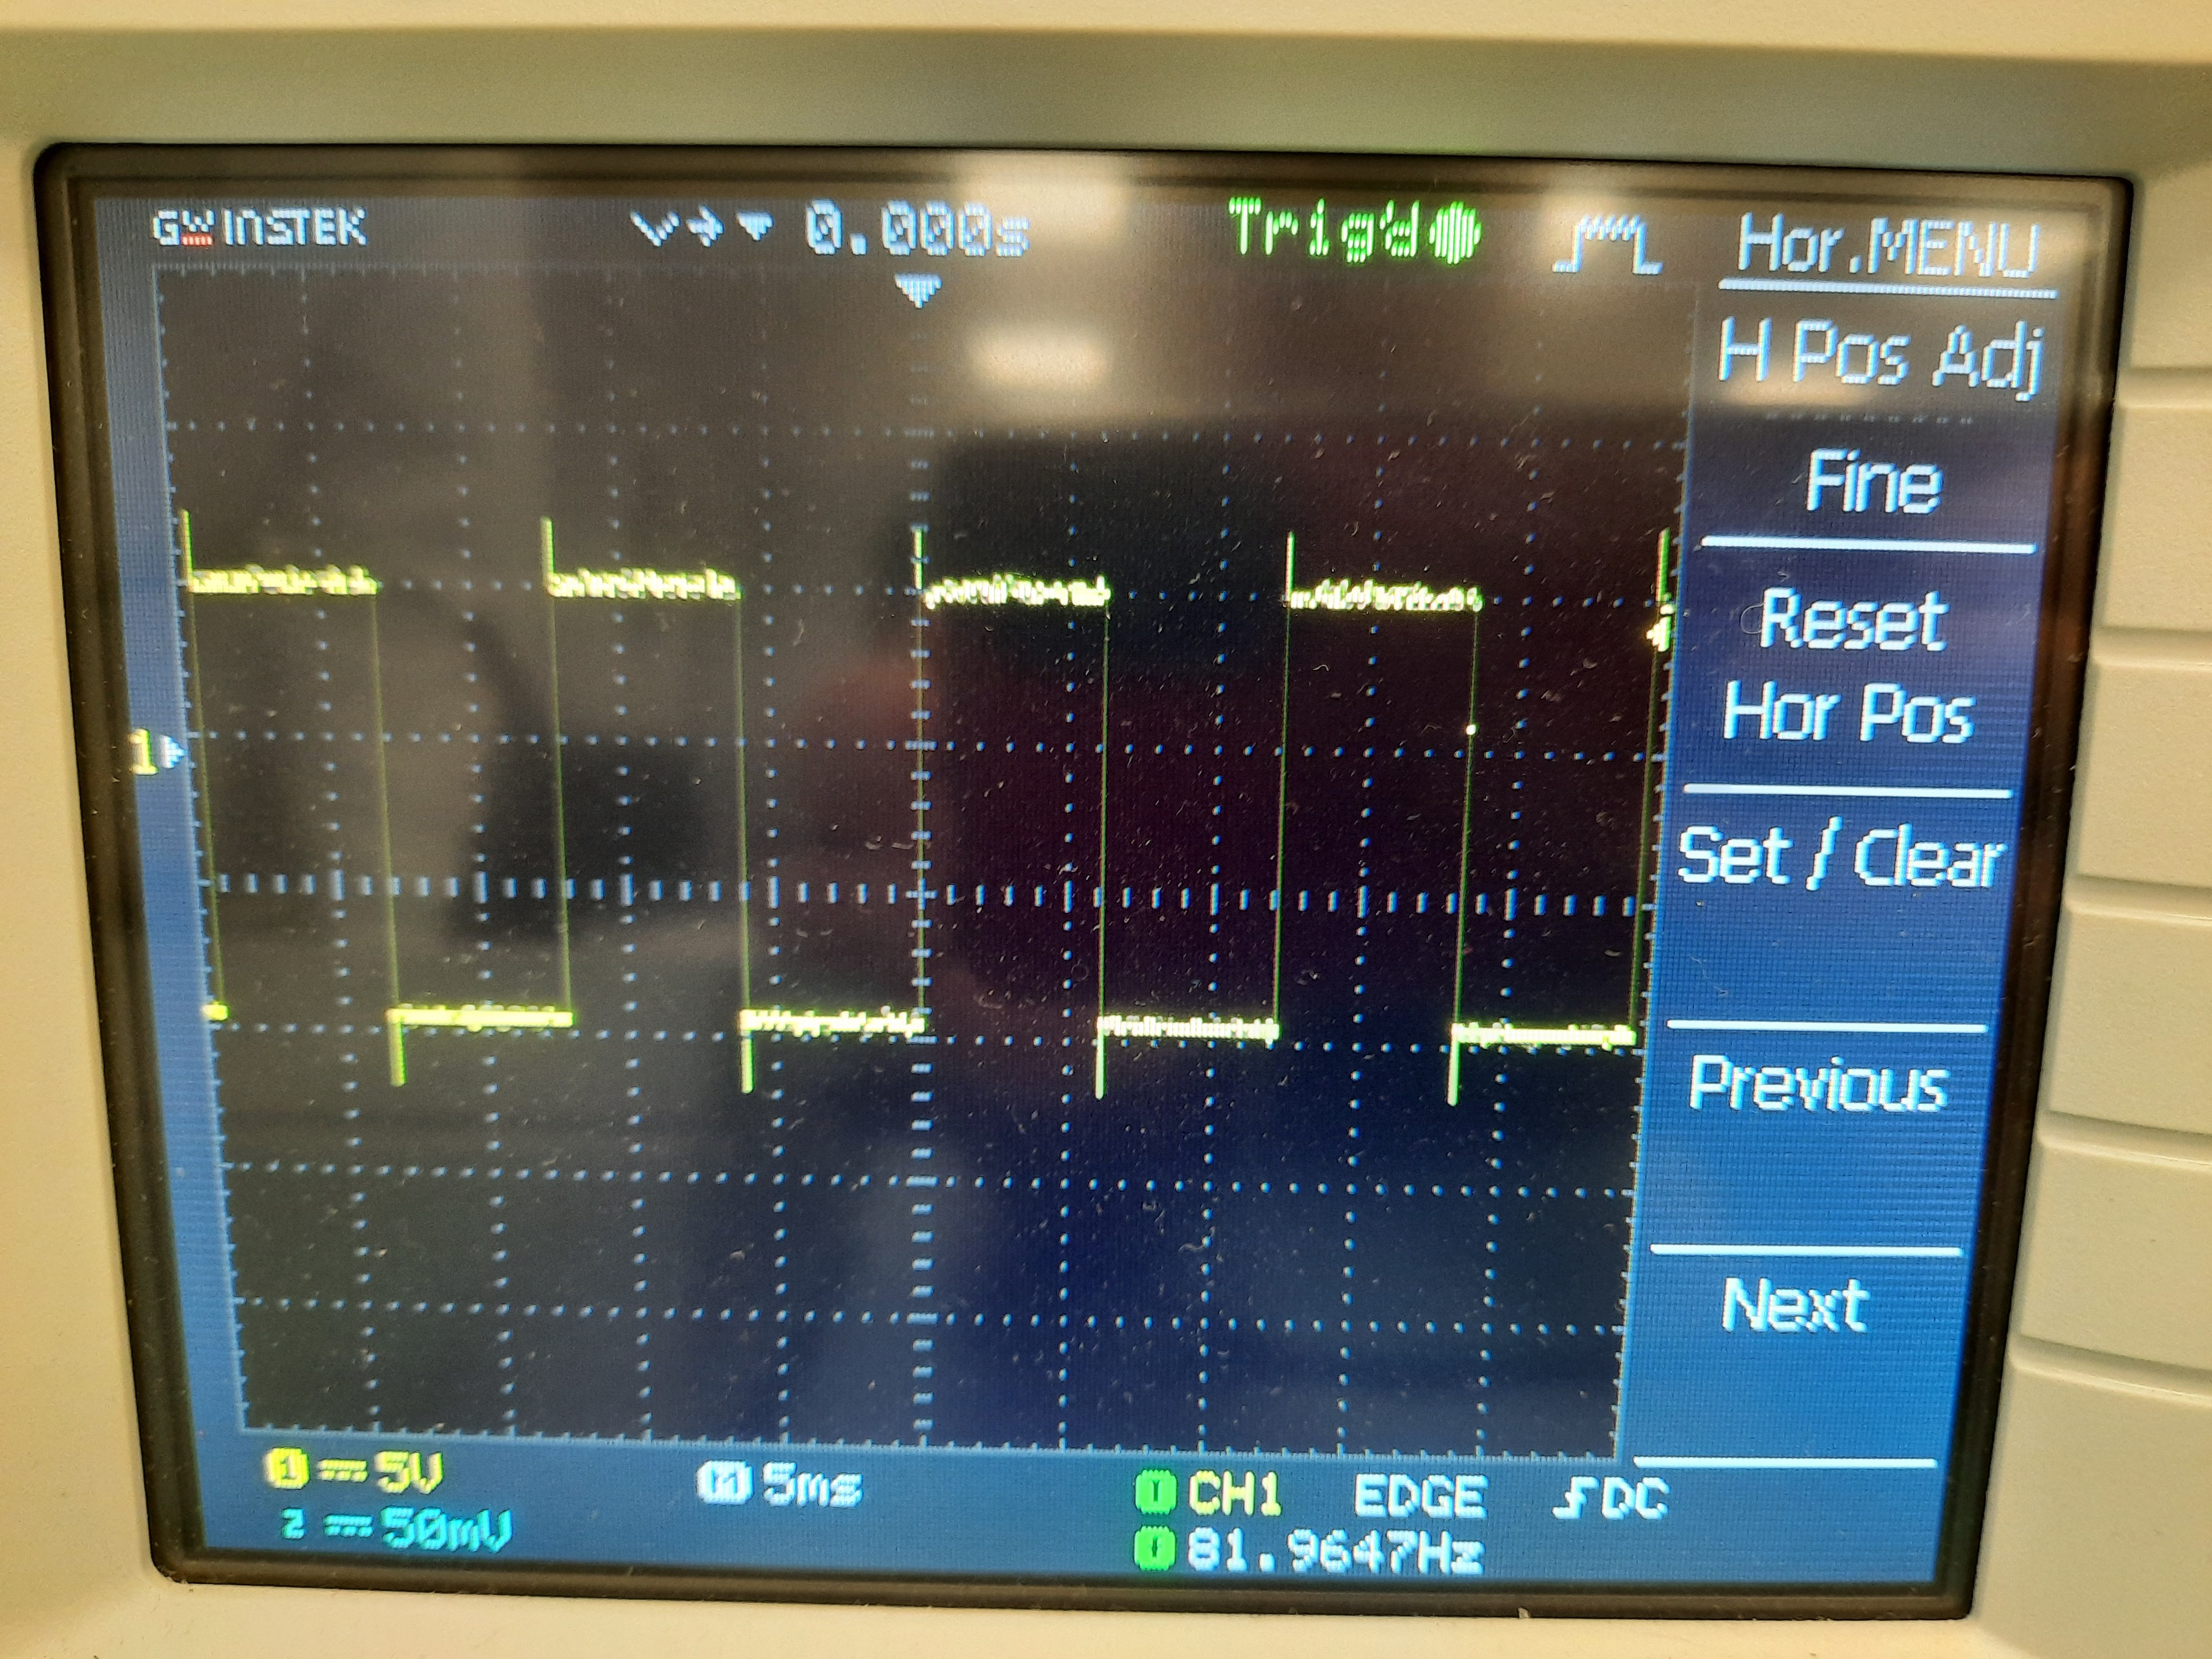
\includegraphics[width=.95\linewidth]{square_wave_2.jpg}
\end{subfigure}
\caption{Square waves generated}
\end{figure}   

\begin{figure}
\begin{subfigure}{0.5\textwidth}
\centering
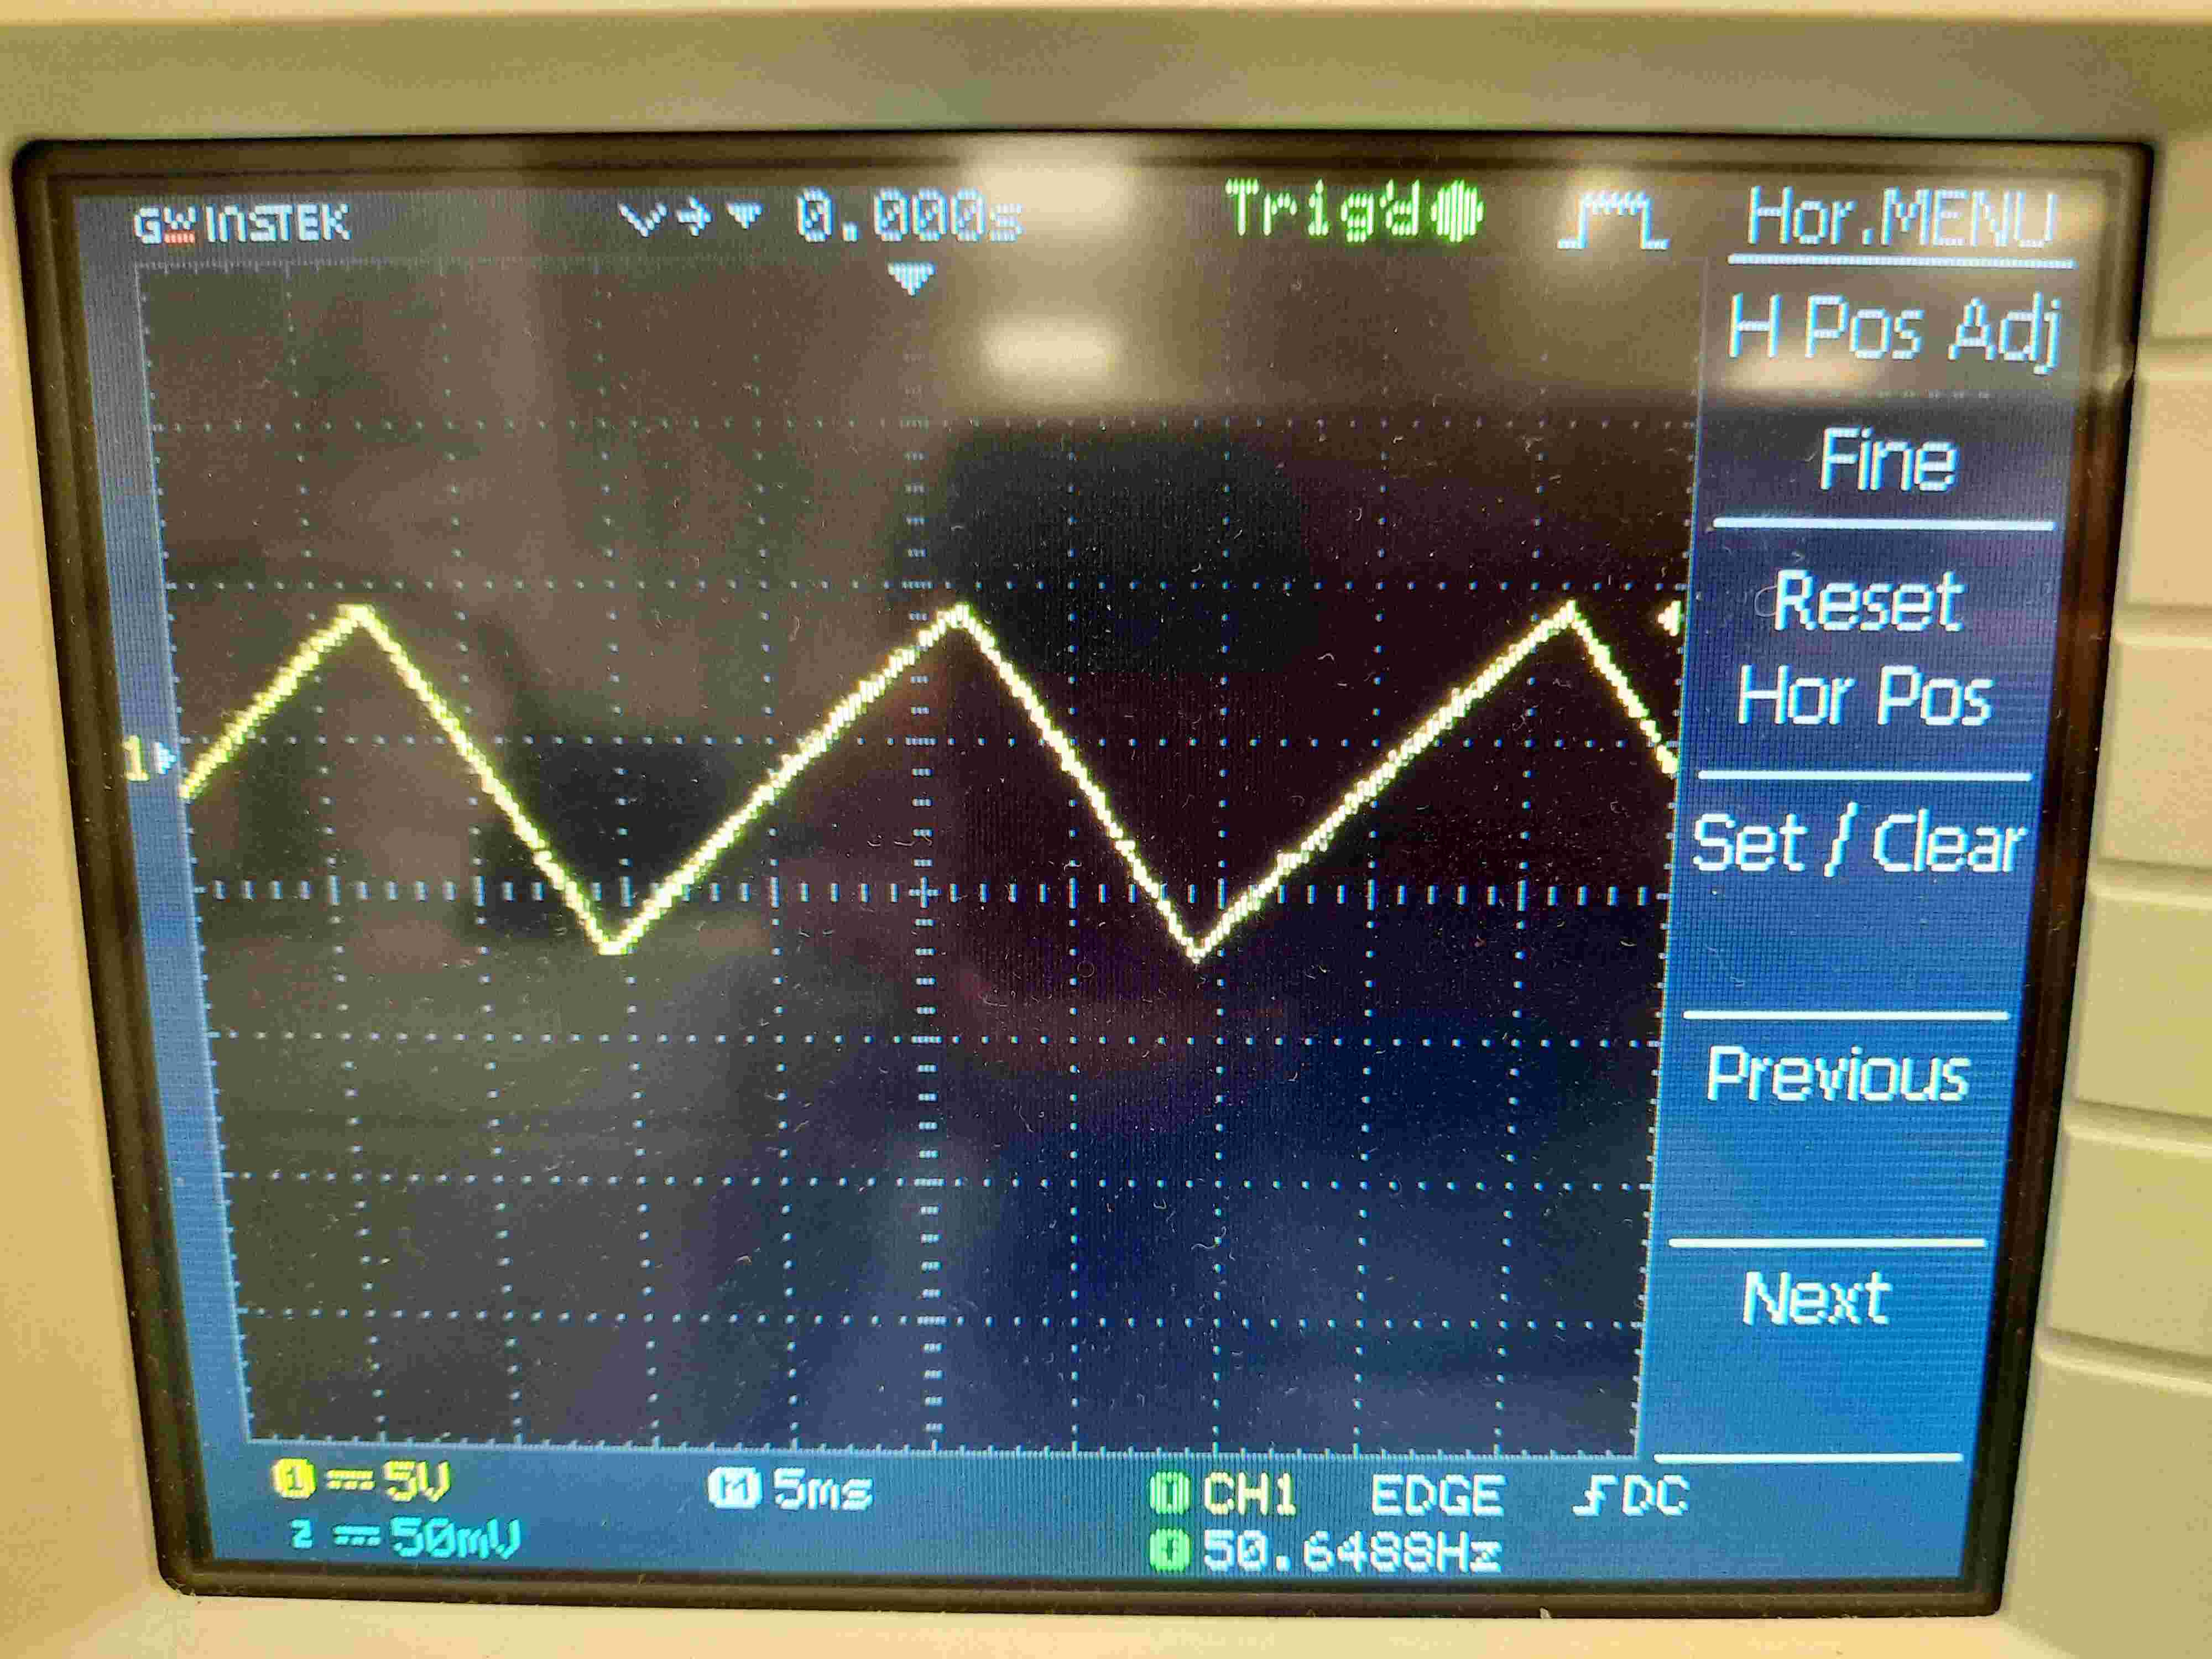
\includegraphics[width=.95\linewidth]{triangle_wave_1.jpg}
\end{subfigure}%
\begin{subfigure}{0.5\textwidth}
\centering
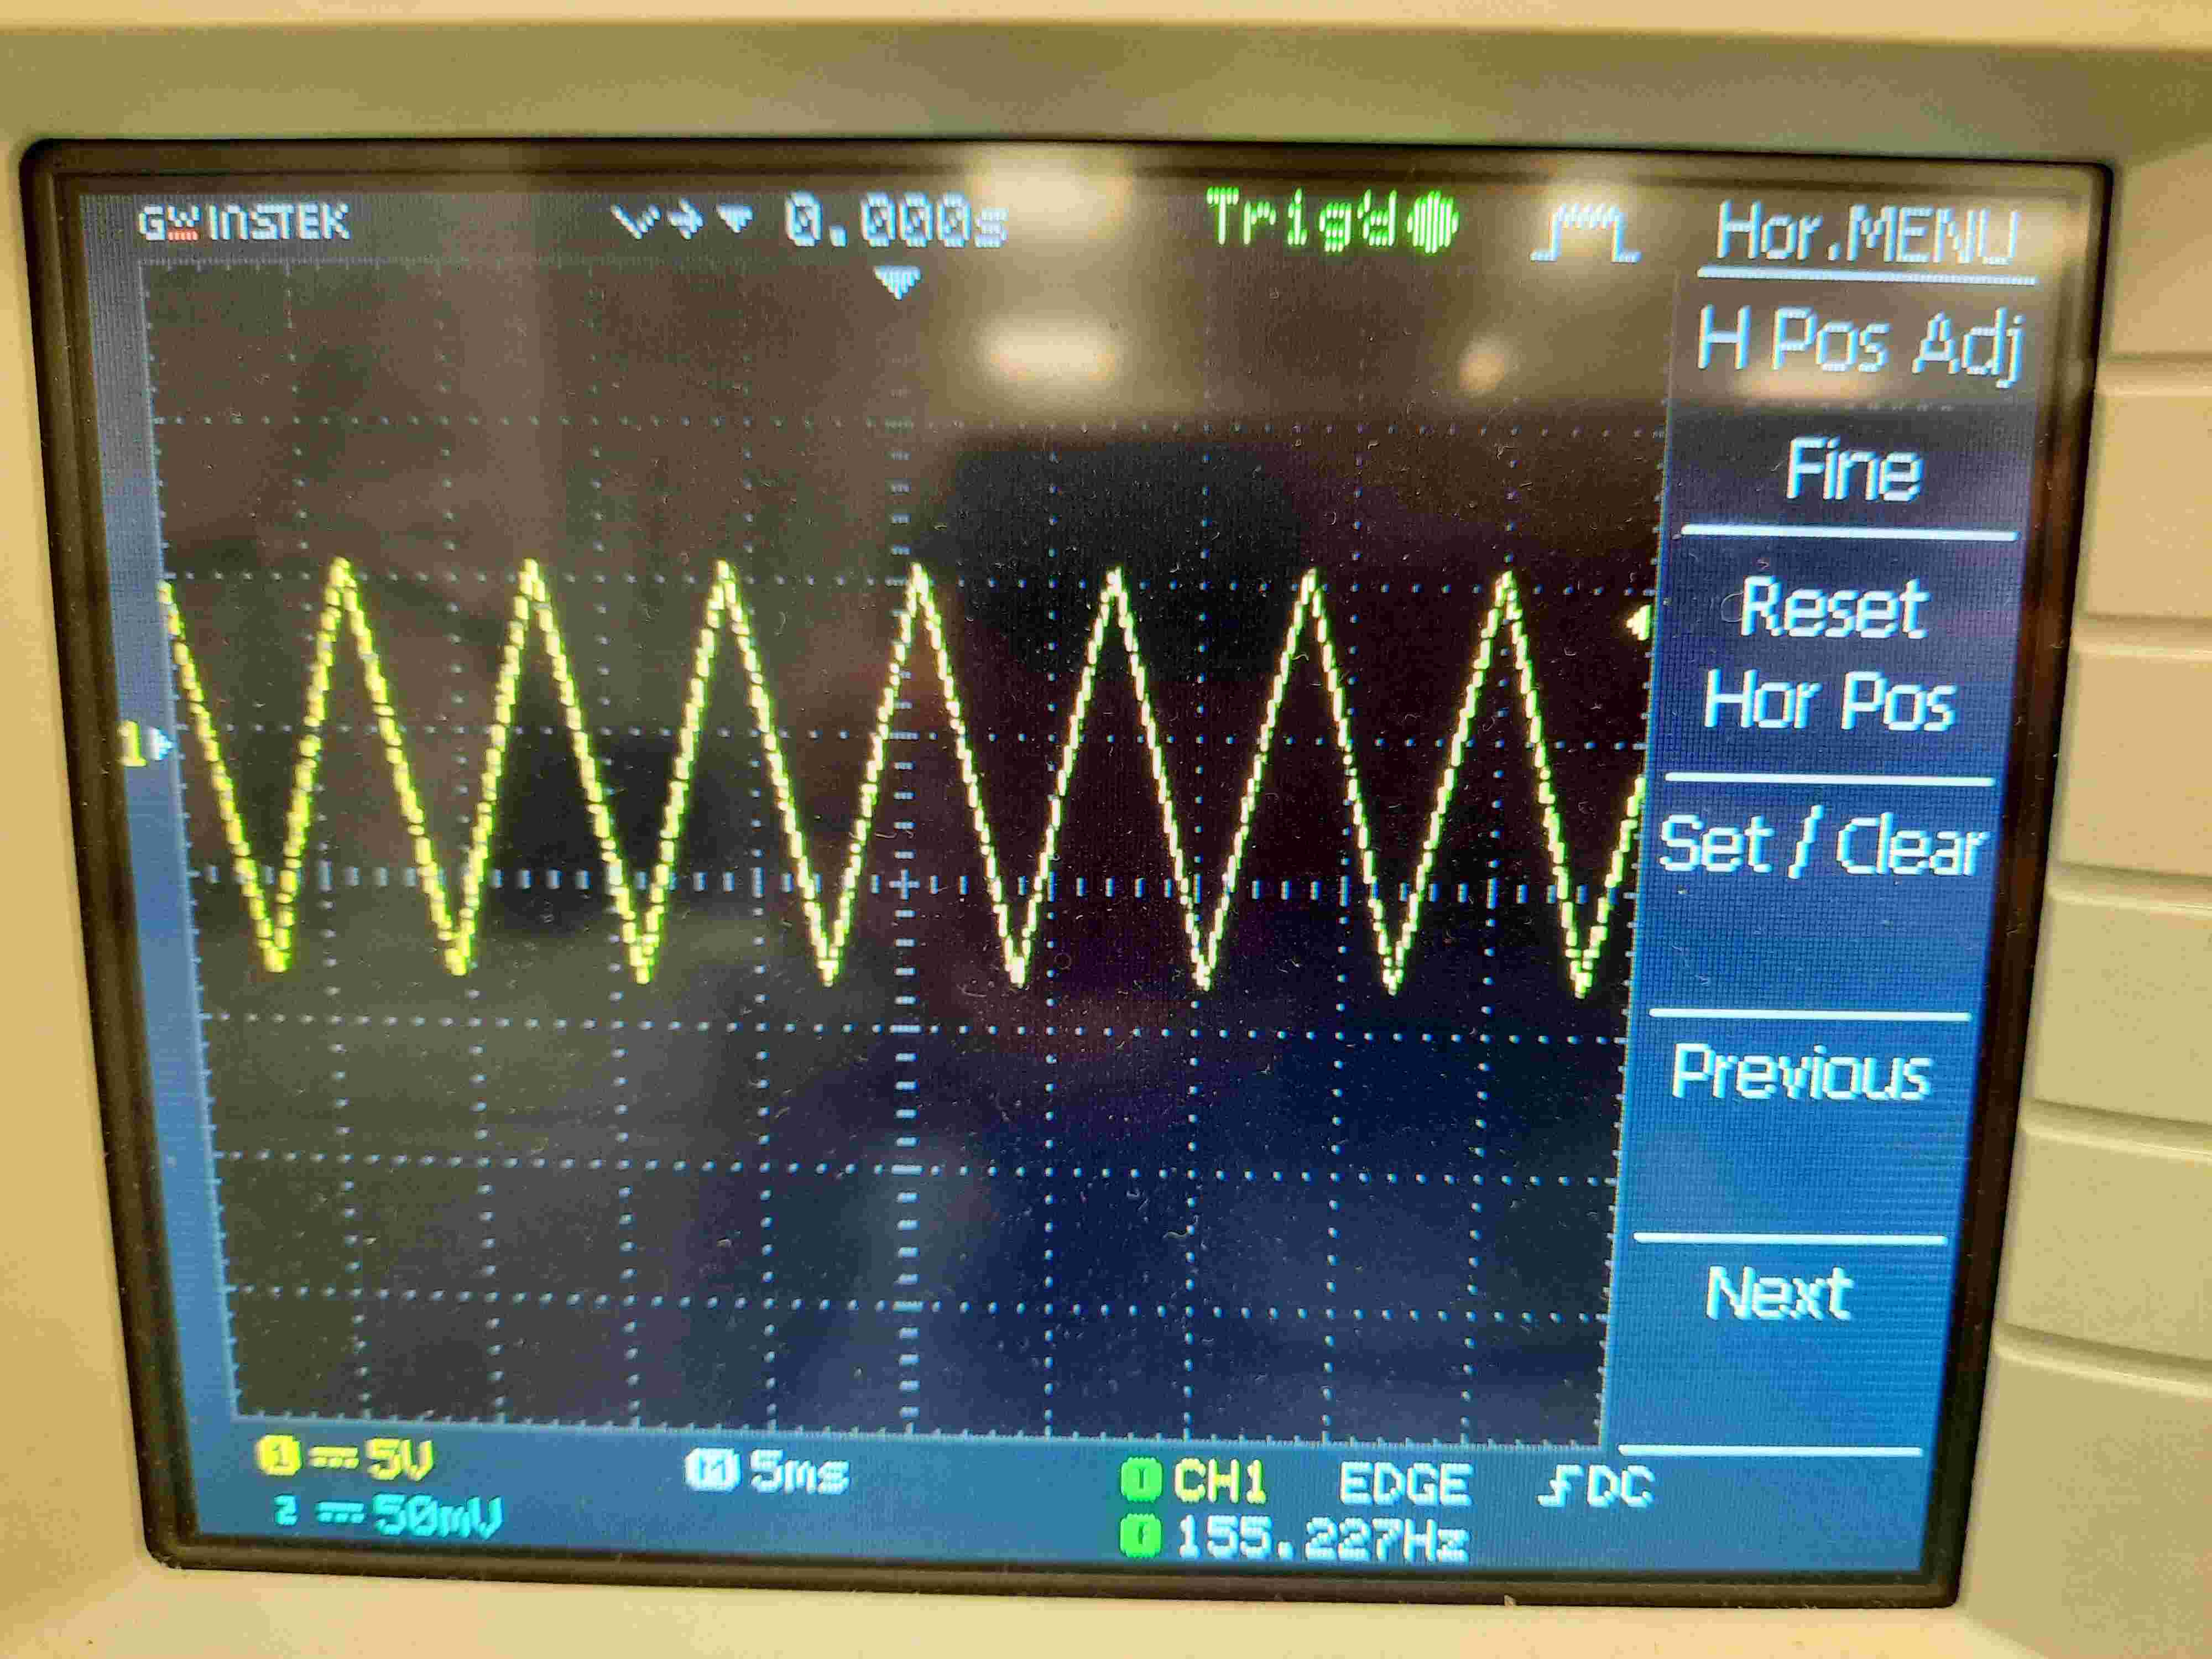
\includegraphics[width=.95\linewidth]{triangle_wave_2.jpg}
\end{subfigure}
\caption{Triangle waves generated}
\end{figure}    
    
\end{itemize}
\section{RESULTS [15 points]}
During this experiment, all of the theoretical predictions made from boolean algebra axioms and truth tables turned out to be true. By using integrated circuits containing AND, OR, and NOT gates, different boolean functions were implemented. Besides that, we practiced the most basic prototyping on breadboard and applied our electronics knowledge. 

\section{DISCUSSION [25 points]} 
To elaborate on what we have done during experiment, a few things can be pointed out. First of all, we were required to study the datasheets of the 74 series ICs. The datasheets presented in the experiment booklet contained just the pinout diagrams and function tables. We noticed that the voltage supply and ground pins are in the same locations for most of the chips, and the outputs were directly below the inputs, a standard design choice which made it easier to quickly memorize the pins. Secondly, we learned how to use C.A.D.E.T., breadboards on it, wires and classical debugging with a multimeter. The latter was useful to check for connectivity and measuring high-low logic levels, when a pin was tricky to be accessed and connected to high/low probes. We configured SPDT switches to act as high/low inputs, while keeping in mind that it can be used in other different ways, such as switching between two signals. Although in this experiment there was no need for pull-up or pull-down resistors, we learned how to build desired resistance with a potentiometer. The oscilloscope and function generator were studied, and although digital electronics use only two voltage levels and a logic analyzer is a more practical device, on higher clock frequencies the square wave degrades and using oscilloscope in solving problems gives a full picture of what is going on.

\section{CONCLUSION [10 points]}
There were difficulties in getting used to the laboratory setup, we had problems primarily with the breadboards, function generator and oscilloscope. The breadboards were unusual by having power lines cut in the middle, and on our first tries of building circuits we were confused of getting high impedance state on output. The problem was not immediately obvious. Then the experiment went fine until the last part, where we were getting nothing meaningful on the oscilloscope display. We had no confidence in whether it was our wiring, function generator parameters or oscilloscope itself. With the help of professor, we found out that the function generator on our C.A.D.E.T. was broken and we tried other set instead. Overall, the experiment went exciting because we learned the practical side of designing digital circuitry.

\newpage
\addcontentsline{toc}{section}{\numberline {}REFERENCES}

\bibliographystyle{unsrt}
\bibliography{reference}

\end{document}

